% !TeX program = xelatex
% !TeX encoding = UTF-8
\documentclass[12pt,openany,oneside]{book}

\usepackage[a4paper,top=23mm,bottom=25mm,left=25mm,right=25mm,headheight=17pt]{geometry}
\usepackage{amsmath,amssymb,amsfonts,mathtools,bm}
\usepackage{amsthm}
\usepackage{booktabs,longtable,array,multirow,tabularx}
\usepackage{graphicx}
\graphicspath{{figures/}}
\usepackage{xcolor}
\usepackage{tikz}
\usetikzlibrary{arrows.meta,positioning,calc,fit,shapes.geometric,decorations.pathreplacing,matrix,patterns,3d}
\usepackage[most]{tcolorbox}
\usepackage{enumitem}
\usepackage{listings}
\usepackage{caption}
\usepackage{subcaption}
\usepackage{float}
\usepackage{fancyhdr}
\usepackage{titlesec}
\usepackage{setspace}
\usepackage{microtype}
\usepackage{hyperref}
\usepackage{xepersian}

\IfFontExistsTF{Amiri}
  {\settextfont[Scale=1.08]{Amiri}\setdigitfont{Amiri}}
  {\settextfont[Scale=1.05]{Noto Naskh Arabic}\setdigitfont{Noto Naskh Arabic}}
\IfFontExistsTF{DejaVu Serif}
  {\setlatintextfont{DejaVu Serif}}
  {\setlatintextfont{Latin Modern Roman}}
\IfFontExistsTF{DejaVu Sans Mono}
  {\setmonofont{DejaVu Sans Mono}}
  {\setmonofont{Latin Modern Mono}}

\definecolor{DeepBlue}{HTML}{163A5F}
\definecolor{Accent}{HTML}{B34B35}
\definecolor{SoftBlue}{HTML}{EAF2F8}
\definecolor{SoftGold}{HTML}{FFF6DF}
\definecolor{SoftGreen}{HTML}{EAF7EF}
\definecolor{SoftRed}{HTML}{FCEDEC}
\definecolor{SoftGray}{HTML}{F4F5F6}
\definecolor{CodeGray}{HTML}{F7F7F7}

\hypersetup{
  colorlinks=true,
  linkcolor=DeepBlue,
  citecolor=Accent,
  urlcolor=Accent,
  pdftitle={پردازش تصویر در دهه آینده ـ فصل دوازدهم: مدل‌های مولد تصویر},
  pdfauthor={جزوه درس کارشناسی ارشد}
}

\setstretch{1.22}
\setlength{\parskip}{0.35em}
\setlength{\parindent}{1.3em}
\setlist[itemize]{itemsep=0.25em,topsep=0.35em,leftmargin=9mm}
\setlist[enumerate]{itemsep=0.25em,topsep=0.35em,leftmargin=10mm}

\pagestyle{fancy}
\fancyhf{}
\fancyhead[R]{\small\thepage}
\fancyhead[L]{\small\nouppercase{\leftmark}}
\renewcommand{\headrulewidth}{0.4pt}

\titleformat{\chapter}[display]
  {\normalfont\huge\bfseries\color{DeepBlue}}
  {\filleft\Large فصل \thechapter}
  {8pt}
  {\filright}
\titleformat{\section}{\Large\bfseries\color{DeepBlue}}{\thesection}{0.7em}{}
\titleformat{\subsection}{\large\bfseries\color{Accent}}{\thesubsection}{0.7em}{}
\titleformat{\subsubsection}{\normalsize\bfseries\color{DeepBlue}}{\thesubsubsection}{0.7em}{}

\newtheorem{definition}{تعریف}[chapter]
\newtheorem{theorem}{قضیه}[chapter]
\newtheorem{proposition}{گزاره}[chapter]
\newtheorem{lemma}{لم}[chapter]
\newtheorem{example}{مثال}[chapter]
\newtheorem{remark}{نکته}[chapter]
\newtheorem{corollary}{نتیجه}[chapter]
\renewcommand{\proofname}{اثبات}

\newtcolorbox{learningbox}{colback=SoftBlue,colframe=DeepBlue,title=اهداف یادگیری,fonttitle=\bfseries,breakable,enhanced}
\newtcolorbox{keybox}[1][]{colback=SoftGold,colframe=Accent,title={#1},fonttitle=\bfseries,breakable,enhanced}
\newtcolorbox{futurebox}{colback=SoftGreen,colframe=green!50!black,title=پل به دهه آینده,fonttitle=\bfseries,breakable,enhanced}
\newtcolorbox{warningbox}{colback=SoftRed,colframe=red!65!black,title=خطای رایج,fonttitle=\bfseries,breakable,enhanced}
\newtcolorbox{workshopbox}[1][]{colback=SoftGray,colframe=black!55,title={کارگاه کد و آزمایش: #1},fonttitle=\bfseries,breakable,enhanced}
\newtcolorbox{researchbox}[1][]{colback=white,colframe=purple!65!black,title={خواندن مقاله و استاندارد: #1},fonttitle=\bfseries,breakable,enhanced}
\newtcolorbox{videobox}{colback=white,colframe=DeepBlue,title=تقسیم پیشنهادی ویدئوهای ۱۵ دقیقه‌ای,fonttitle=\bfseries,breakable,enhanced}
\newtcolorbox{proofbox}[1][]{colback=white,colframe=DeepBlue!65,title={مسیر اثبات: #1},fonttitle=\bfseries,breakable,enhanced}
\newtcolorbox{codecontract}{colback=SoftBlue,colframe=Accent,title=قرارداد میان ریاضیات و کد,fonttitle=\bfseries,breakable,enhanced}
\newtcolorbox{summarybox}{colback=SoftBlue,colframe=DeepBlue,title=جمع‌بندی فصل,fonttitle=\bfseries,breakable,enhanced}
\newtcolorbox{goalbox}{colback=SoftBlue,colframe=DeepBlue,title=هدف فصل,fonttitle=\bfseries,breakable,enhanced}
\newtcolorbox{principlebox}{colback=SoftGold,colframe=Accent,title=اصل راهنما,fonttitle=\bfseries,breakable,enhanced}
\newtcolorbox{algorithmbox}[1]{colback=SoftGray,colframe=DeepBlue,title={#1},fonttitle=\bfseries,breakable,enhanced}
\newtcolorbox{theorembox}[1]{colback=white,colframe=purple!65!black,title={#1},fonttitle=\bfseries,breakable,enhanced}
\newtcolorbox{applicationbox}[1][]{colback=SoftGreen,colframe=green!45!black,title={کاربرد مهندسی: #1},fonttitle=\bfseries,breakable,enhanced}
\newtcolorbox{librarybox}[1][]{colback=white,colframe=blue!50!black,title={کتابخانه و ابزار: #1},fonttitle=\bfseries,breakable,enhanced}
\newtcolorbox{diagnosticbox}[1][]{colback=SoftRed,colframe=Accent,title={آزمون تشخیصی: #1},fonttitle=\bfseries,breakable,enhanced}

\newcommand{\R}{\mathbb{R}}
\newcommand{\C}{\mathbb{C}}
\newcommand{\N}{\mathbb{N}}
\newcommand{\Z}{\mathbb{Z}}
\newcommand{\E}{\mathbb{E}}
\newcommand{\Var}{\operatorname{Var}}
\newcommand{\Cov}{\operatorname{Cov}}
\newcommand{\Prob}{\mathbb{P}}
\newcommand{\norm}[1]{\left\lVert #1\right\rVert}
\newcommand{\abs}[1]{\left\lvert #1\right\rvert}
\newcommand{\inner}[2]{\left\langle #1,#2\right\rangle}
\newcommand{\trans}{^{\mathsf T}}
\newcommand{\herm}{^{\mathsf H}}
\newcommand{\inv}{^{-1}}
\newcommand{\vect}[1]{\bm{#1}}
\newcommand{\mat}[1]{\bm{#1}}
\newcommand{\argmin}{\operatorname*{arg\,min}}
\newcommand{\argmax}{\operatorname*{arg\,max}}
\newcommand{\trace}{\operatorname{tr}}
\newcommand{\diag}{\operatorname{diag}}
\newcommand{\rank}{\operatorname{rank}}
\newcommand{\softmax}{\operatorname{softmax}}
\newcommand{\ReLU}{\operatorname{ReLU}}
\newcommand{\GAP}{\operatorname{GAP}}
\newcommand{\FLOPs}{\operatorname{FLOPs}}
\newcommand{\CE}{\operatorname{CE}}
\newcommand{\BN}{\operatorname{BN}}
\newcommand{\LN}{\operatorname{LN}}
\newcommand{\GN}{\operatorname{GN}}
\newcommand{\IN}{\operatorname{IN}}
\newcommand{\sigmoid}{\operatorname{sigmoid}}

\lstset{
  language=Python,
  basicstyle=\footnotesize\ttfamily\color{black},
  columns=fullflexible,
  keepspaces=true,
  backgroundcolor=\color{CodeGray},
  frame=single,
  rulecolor=\color{black!25},
  numbers=left,
  numberstyle=\tiny,
  breaklines=true,
  showstringspaces=false,
  keywordstyle=\bfseries\color{DeepBlue},
  commentstyle=\itshape\color{black!65},
  stringstyle=\color{Accent},
  tabsize=4
}



\newcommand{\KL}{\operatorname{KL}}
\newcommand{\JS}{\operatorname{JS}}
\newcommand{\ELBO}{\operatorname{ELBO}}
\newcommand{\FID}{\operatorname{FID}}
\newcommand{\KID}{\operatorname{KID}}
\newcommand{\MMD}{\operatorname{MMD}}
\newcommand{\supp}{\operatorname{supp}}
\newcommand{\sg}{\operatorname{sg}}
\newcommand{\logit}{\operatorname{logit}}

\begin{document}

\begin{titlepage}
\centering
\vspace*{0.8cm}
{\color{DeepBlue}\rule{0.9\textwidth}{1.1pt}}\\[0.9cm]
{\Huge\bfseries پردازش تصویر در دهه آینده\\[0.3cm]}
{\LARGE\bfseries از عمق ریاضیات تا مهندس حرفه‌ای\\[0.8cm]}
{\Large کتاب ـ جزوه درس کارشناسی ارشد و آزمایشگاه پژوهش‌محور\\[0.9cm]}

\begin{tikzpicture}[node distance=8mm]
\node[draw=DeepBlue,very thick,rounded corners=3mm,fill=SoftBlue,
      minimum width=13.4cm,minimum height=5.5cm,text width=12.8cm,align=center] (a)
{\Large\bfseries فصل دوازدهم\\[2mm]
\large مدل‌های مولد تصویر\\[1mm]
\normalsize از خودرمزگذار و استنباط واریاسیونی تا \lr{VAE}، \lr{VQ-VAE}،
\lr{GAN}، مدل‌های خودرگرسیو، جریان‌های نرمال‌ساز، مدل‌های انرژی‌محور و مولدهای توکنی جدید};
\node[below=7mm of a,align=center,text width=12.8cm] {
هدف فصل فقط تولید چند تصویر چشم‌نواز نیست. دانشجو باید بداند مدل چه توزیعی را می‌آموزد،
تابع هدف چه فاصله یا کرانی را کمینه می‌کند، نمونه‌گیری چه هزینه‌ای دارد، فروپاشی چگونه تشخیص داده می‌شود
و چرا یک معیار عددی یا چند تصویر منتخب برای ادعای موفقیت کافی نیست.};
\end{tikzpicture}

\vfill
{\large نسخه تفصیلی درس ـ تابستان ۱۴۰۵ / ۲۰۲۶}\\[0.4cm]
{\normalsize قابل کامپایل با \lr{TeX Live + TeXstudio + XeLaTeX}}\\[0.8cm]
{\color{DeepBlue}\rule{0.9\textwidth}{1.1pt}}
\end{titlepage}

\frontmatter

\chapter*{یادداشت روش‌شناختی فصل دوازدهم}
\addcontentsline{toc}{chapter}{یادداشت روش‌شناختی فصل دوازدهم}
فصل‌های پیشین به استخراج ویژگی، شبکه‌های کانولوشنی و نمایش‌های خودنظارتی پرداختند. در آن فصل‌ها، مدل عمدتاً
یک نگاشت پیش‌بین بود: تصویر را می‌گرفت و برچسب، ویژگی یا ماسک می‌ساخت. مدل مولد یک پرسش بنیادی‌تر می‌پرسد:
\textbf{چه سازوکار احتمالاتی می‌تواند خود داده را تولید کند؟} پاسخ این پرسش می‌تواند به‌صورت چگالی صریح،
متغیر نهفته، بازی خصمانه، فاکتورگیری خودرگرسیو، تبدیل وارون‌پذیر یا میدان انرژی بیان شود. این صورت‌بندی‌ها
از نظر تابع هدف، نوع استنباط، کیفیت نمونه، پوشش توزیع و هزینه محاسباتی یکسان نیستند.

در این فصل، اصطلاح «مدل مولد» برای هر شبکه‌ای که تصویری خروجی می‌دهد به‌کار نمی‌رود. یک مدل مولد باید
درباره توزیع داده ادعایی مشخص داشته باشد؛ مثلاً چگالی یا کران درست‌نمایی ارائه کند، نمونه‌های خود را به‌عنوان
pushforward یک توزیع پایه تعریف کند، یا از طریق یک منتقد فاصله میان توزیع داده و مدل را کاهش دهد. بنابراین
هر معماری با پنج پرسش سنجیده می‌شود:
\begin{enumerate}
\item متغیر تصادفی پایه و فضای نمونه چیست؟
\item مدل چگالی صریح دارد یا فقط نمونه تولید می‌کند؟
\item تابع هدف دقیقاً چه کمیتی را کمینه یا بیشینه می‌کند؟
\item استنباط، بازسازی و نمونه‌گیری چگونه انجام می‌شوند؟
\item شکست غالب آن چیست و با چه آزمونی آشکار می‌شود؟
\end{enumerate}

\begin{goalbox}
این فصل شش خروجی هم‌زمان دارد:
\begin{enumerate}
\item \textbf{مبانی احتمال:} دانشجو بتواند درست‌نمایی، واگرایی، pushforward، تغییر متغیر و متغیر نهفته را با نمادگذاری دقیق بنویسد.
\item \textbf{استنباط واریاسیونی:} دانشجو بتواند \lr{ELBO} را استخراج و شکاف واریاسیونی، بازپارامتردهی و فروپاشی پسین را تحلیل کند.
\item \textbf{بازی خصمانه:} دانشجو بتواند تمایزگر بهینه، ارتباط \lr{GAN} با \lr{JS}، نسخه غیر اشباع، \lr{WGAN} و جریمه گرادیان را توضیح دهد.
\item \textbf{مدل‌های چگالی صریح:} دانشجو بتواند فاکتورگیری خودرگرسیو و فرمول تغییر متغیر در جریان‌های نرمال‌ساز را پیاده‌سازی کند.
\item \textbf{توان مهندسی:} دانشجو بتواند نسخه آموزشی \lr{VAE}، \lr{VQ-VAE}، \lr{GAN}، \lr{WGAN-GP}، \lr{PixelCNN} و \lr{RealNVP} را اجرا و عیب‌یابی کند.
\item \textbf{ارزیابی صادقانه:} دانشجو میان کیفیت، پوشش، درست‌نمایی، حفظ‌کردن داده، وفاداری شرطی و هزینه تمایز بگذارد.
\end{enumerate}
\end{goalbox}

\begin{figure}[H]
\centering
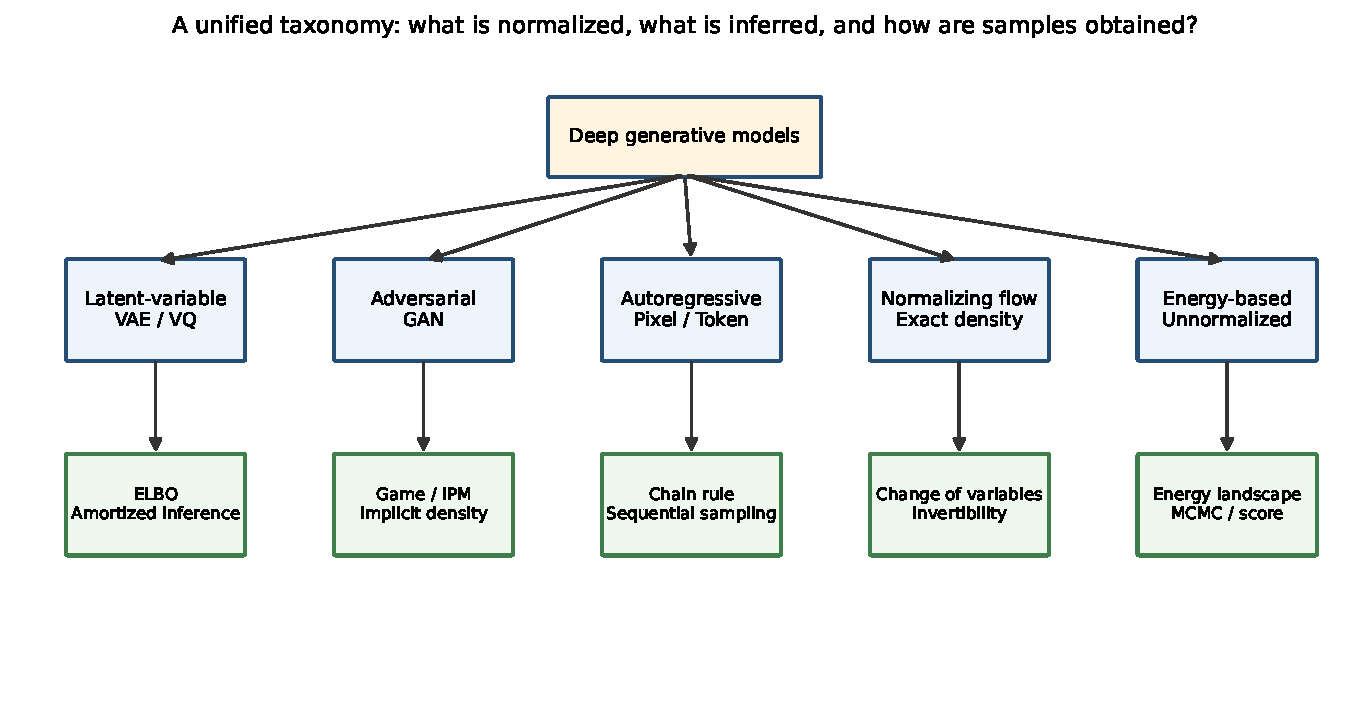
\includegraphics[width=0.98\textwidth]{fig12_01_taxonomy.pdf}
\caption{رده‌بندی یکپارچه مدل‌های مولد عمیق. تفاوت اصلی فقط معماری نیست؛ بلکه نوع نرمال‌سازی، استنباط، تابع هدف و سازوکار نمونه‌گیری است.}
\label{fig:gen-taxonomy}
\end{figure}

\chapter*{نقشه فشرده فصل}
\addcontentsline{toc}{chapter}{نقشه فشرده فصل}
\begin{longtable}{p{38mm}p{101mm}}
\toprule
محور & پرسش و خروجی آموزشی \\
\midrule
احتمال مولد & $p_{\rm data}$، $p_\theta$، pushforward، چگالی صریح و ضمنی چه تفاوتی دارند؟ \\
خودرمزگذار & بازسازی چه نسبتی با \lr{PCA}، منیفلد و مدل مولد دارد؟ \\
\lr{VAE} & \lr{ELBO} چگونه استخراج می‌شود و بازپارامتردهی چگونه گرادیان را از نمونه‌گیری عبور می‌دهد؟ \\
نسخه‌های واریاسیونی & $\beta$-VAE، \lr{IWAE}، \lr{WAE}، \lr{InfoVAE} و مدل‌های سلسله‌مراتبی کدام بخش مدل را تغییر می‌دهند؟ \\
کوانتیزه‌سازی & \lr{VQ-VAE/VQGAN} چگونه تصویر را به الفبای گسسته تبدیل می‌کند و codebook collapse چیست؟ \\
\lr{GAN} & تمایزگر بهینه چه نسبت چگالی‌ای می‌آموزد و چرا آموزش یک بازی دینامیکی است؟ \\
پایداری خصمانه & \lr{WGAN}، قید Lipschitz، gradient penalty، spectral normalization، \lr{R1} و \lr{TTUR} چه می‌کنند؟ \\
معماری‌های GAN & \lr{DCGAN}، شرطی، \lr{pix2pix}، \lr{CycleGAN}، \lr{BigGAN} و \lr{StyleGAN1--3} چه پیشرفت‌هایی دارند؟ \\
خودرگرسیو & قاعده زنجیره چگونه چگالی دقیق می‌دهد و چرا نمونه‌گیری پیکسلی کند است؟ \\
مولدهای توکنی & \lr{VQGAN+Transformer}، \lr{MaskGIT}، \lr{LlamaGen}، \lr{VAR} و tokenizerهای فشرده چه مبادله‌ای دارند؟ \\
جریان‌ها & تغییر متغیر، coupling، \lr{RealNVP}، \lr{Glow}، \lr{MAF/IAF} و جریان پیوسته چگونه درست‌نمایی دقیق می‌دهند؟ \\
انرژی & چرا ثابت نرمال‌سازی دشوار است و فاز مثبت/منفی، \lr{MCMC} و score matching چه نقشی دارند؟ \\
ارزیابی & \lr{ELBO}، bits/dim، \lr{FID}، \lr{KID}، precision/recall، حفظ داده و ارزیابی انسانی چگونه ترکیب می‌شوند؟ \\
کتابخانه‌ها & PyTorch، \lr{Diffusers}، \lr{MMagic}، مخزن \lr{StyleGAN3} و ابزارهای معیار در چه سطحی استفاده می‌شوند؟ \\
پل به فصل بعد & جریان تطبیقی، score و مدل‌های نهفته چگونه به مدل‌های انتشار و انتقال پیوسته می‌رسند؟ \\
\bottomrule
\end{longtable}

\tableofcontents
\mainmatter
\setcounter{chapter}{11}
\chapter{مدل‌های مولد تصویر}

\begin{learningbox}
در پایان فصل، دانشجو باید بتواند:
\begin{itemize}
\item مدل مولد صریح و ضمنی را تعریف و برای هر خانواده مسیر نمونه‌گیری را رسم کند؛
\item واگرایی‌های \lr{KL} و \lr{JS}، فاصله Wasserstein و \lr{IPM} را از منظر بهینه‌سازی مقایسه کند؛
\item \lr{ELBO}، KL گاوسی و برآوردگر بازپارامتردهی را استخراج کند؛
\item فروپاشی پسین و فروپاشی codebook را با معیارهای عددی تشخیص دهد؛
\item تمایزگر بهینه GAN و مقدار تابع هدف در آن را اثبات کند؛
\item \lr{WGAN-GP} و spectral normalization را برای قید Lipschitz توضیح دهد؛
\item یک masked convolution علّی و یک coupling وارون‌پذیر بنویسد؛
\item معیارهای \lr{FID/KID} را از آمار ویژگی‌ها محاسبه و محدودیت آن‌ها را بیان کند؛
\item یک پروتکل آزمایش منصفانه با seed، split، تعداد نمونه ثابت، بازه اطمینان و nearest-neighbor audit طراحی کند.
\end{itemize}
\end{learningbox}

\section{مدل مولد دقیقاً چیست؟}
فرض کنید تصاویر مشاهده‌شده نمونه‌هایی مستقل از توزیع ناشناخته $p_{\rm data}(\vect x)$ باشند. هدف مدل مولد، ساخت
خانواده‌ای پارامتری $p_\theta$ یا یک سازوکار نمونه‌گیری $G_\theta$ است که رفتار توزیعی داده را تقریب بزند.
این هدف با طبقه‌بندی تفاوت دارد: در طبقه‌بندی فقط مرز تصمیم مهم است، اما در تولید باید احتمال یا جرم تمام ناحیه‌های
معتبر فضا توصیف شود. اگر مدل فقط چند نمونه بسیار زیبا تولید کند ولی بخش بزرگی از حالت‌های واقعی را نادیده بگیرد،
توزیع را نیاموخته است.

\subsection{سه هدف متفاوت که نباید مخلوط شوند}
\begin{enumerate}
\item \textbf{برآورد چگالی:} برای ورودی $\vect x$ مقدار $p_\theta(\vect x)$ یا کرانی بر آن محاسبه شود.
\item \textbf{نمونه‌گیری:} بتوان $\vect x\sim p_\theta$ تولید کرد؛ حتی اگر چگالی صریح ناشناخته باشد.
\item \textbf{استنباط نهفته:} برای تصویر مشاهده‌شده، نمایش $\vect z$ یا توزیع پسین $p_\theta(\vect z\mid\vect x)$ به‌دست آید.
\end{enumerate}
خانواده‌ها در این سه توانایی متفاوت‌اند. جریان نرمال‌ساز، چگالی و استنباط دقیق دارد؛ GAN نمونه‌گیری سریع اما چگالی
ضمنی دارد؛ مدل خودرگرسیو درست‌نمایی دقیق اما نمونه‌گیری ترتیبی دارد؛ VAE استنباط سریع و یک کران واریاسیونی دارد.

\subsection{Pushforward یک توزیع پایه}
اگر $\vect z\sim p_Z$ و $\vect x=G_\theta(\vect z)$ باشد، توزیع مدل pushforward توزیع پایه است:
\begin{equation}
 p_\theta = (G_\theta)_\# p_Z.
\end{equation}
این نماد یعنی برای هر مجموعه اندازه‌پذیر $A$،
\begin{equation}
 p_\theta(A)=p_Z\!\left(G_\theta^{-1}(A)\right).
\end{equation}
اگر بعد نهفته کمتر از بعد تصویر باشد، توزیع روی یک منیفلد کم‌بعد قرار می‌گیرد و لزوماً چگالی لبگ در کل فضای پیکسل ندارد.
این نکته یکی از علت‌های دشواری مقایسه چگالی‌های صریح و مدل‌های ضمنی است.

\begin{figure}[H]
\centering
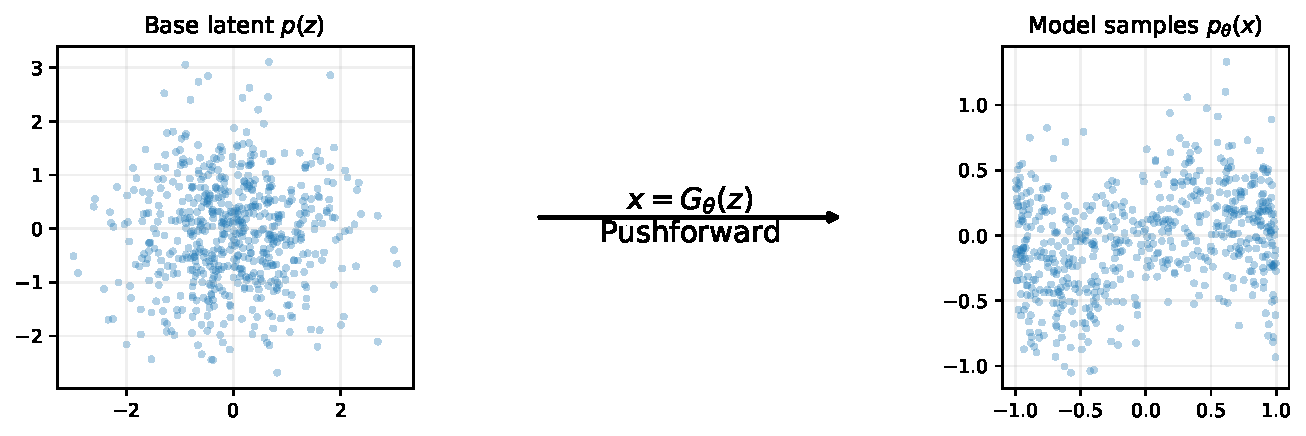
\includegraphics[width=0.95\textwidth]{fig12_02_pushforward.pdf}
\caption{تولید به‌صورت pushforward: توزیع پایه ساده با نگاشت شبکه‌ای به توزیع پیچیده داده منتقل می‌شود.}
\end{figure}

\section{مبانی احتمال و هندسه فاصله میان توزیع‌ها}
\subsection{بیشینه‌سازی درست‌نمایی و آنتروپی متقاطع}
برای داده $\mathcal D=\{\vect x_i\}_{i=1}^n$، برآورد بیشینه درست‌نمایی برابر است با
\begin{equation}
 \hat\theta_{\rm ML}=\argmax_\theta \sum_{i=1}^n \log p_\theta(\vect x_i).
\end{equation}
در حد جمعیت، کمینه‌کردن منفی درست‌نمایی همان کمینه‌کردن
\begin{equation}
 \E_{p_{\rm data}}[-\log p_\theta(\vect x)]
 =H(p_{\rm data})+\KL(p_{\rm data}\Vert p_\theta)
\end{equation}
است. چون آنتروپی داده نسبت به $\theta$ ثابت است، ML جهت \lr{KL} رو به جلو را کمینه می‌کند. این جهت به نواحی دارای
جرم داده حساس است و معمولاً mode-covering توصیف می‌شود، اما تعبیر هندسی آن وابسته به خانواده مدل و ظرفیت آن است.

\subsection{واگرایی KL و نامتقارن بودن آن}
\begin{equation}
 \KL(p\Vert q)=\int p(x)\log\frac{p(x)}{q(x)}\,dx.
\end{equation}
اگر جایی $p(x)>0$ و $q(x)=0$ باشد، مقدار بی‌نهایت می‌شود. جهت معکوس $\KL(q\Vert p)$ رفتار دیگری دارد و ممکن است
به انتخاب یک مد پرچگالی تشویق کند. بنابراین عبارت «کمینه‌کردن KL» بدون ذکر جهت، ناقص است.

\subsection{واگرایی Jensen--Shannon}
با $m=(p+q)/2$،
\begin{equation}
 \JS(p\Vert q)=\frac12\KL(p\Vert m)+\frac12\KL(q\Vert m).
\end{equation}
این کمیت متقارن و کراندار است؛ ولی هنگامی که تکیه‌گاه دو توزیع روی منیفلدهای جدا باشد، می‌تواند اشباع شود و گرادیان
مفیدی برای حرکت منیفلد مولد فراهم نکند.

\subsection{فاصله Wasserstein و IPM}
فاصله انتقال بهینه مرتبه یک
\begin{equation}
 W_1(p,q)=\inf_{\gamma\in\Pi(p,q)}\E_{(x,y)\sim\gamma}\norm{x-y}
\end{equation}
هزینه جابه‌جایی جرم را اندازه می‌گیرد. دوگان کانتوروویچ--روبینشتاین می‌گوید
\begin{equation}
 W_1(p,q)=\sup_{\norm{f}_{L}\le 1}\left[\E_p f(x)-\E_q f(x)\right].
\end{equation}
این فرم پایه WGAN است. خانواده کلی‌تر معیارهای انتگرالی احتمال نیز به صورت
\begin{equation}
 d_{\mathcal F}(p,q)=\sup_{f\in\mathcal F}\left|\E_p f-\E_q f\right|
\end{equation}
تعریف می‌شود. انتخاب کلاس تابع $\mathcal F$ تعیین می‌کند مدل چه تفاوت‌هایی را قابل مشاهده بداند.

\begin{figure}[H]
\centering
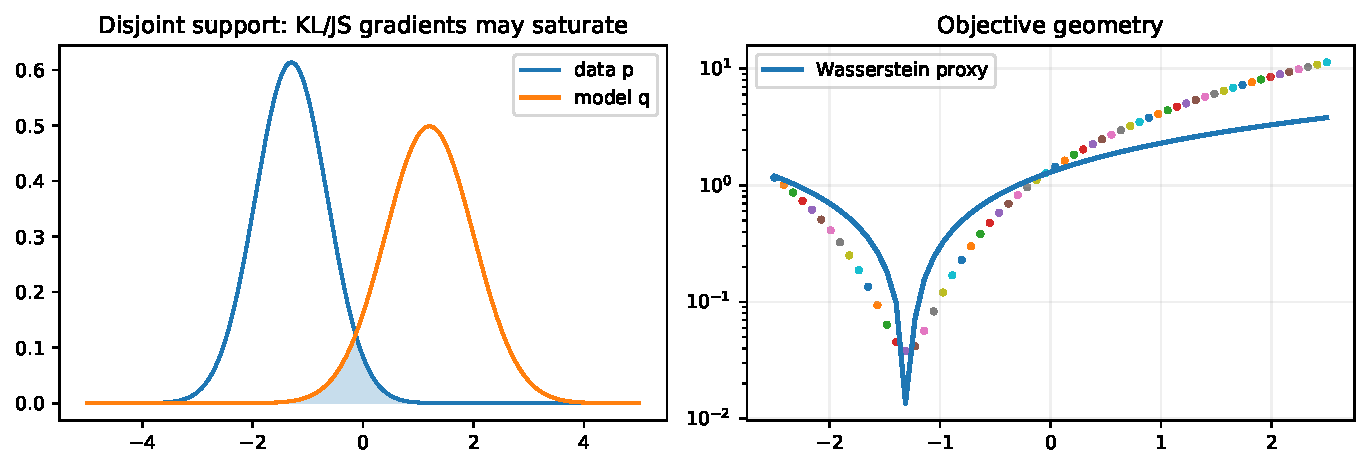
\includegraphics[width=0.96\textwidth]{fig12_03_divergences.pdf}
\caption{تابع فاصله فقط یک عدد گزارش نیست؛ هندسه آن تعیین می‌کند وقتی تکیه‌گاه‌ها جدا هستند چه گرادیانی به مدل برسد.}
\end{figure}

\begin{warningbox}
کوچک بودن یک واگرایی در فضای ویژگی یا تحت یک منتقد محدود، به معنی برابری کامل دو توزیع نیست. هر معیار فقط تفاوت‌هایی را
می‌بیند که کلاس تابع یا استخراج‌گر ویژگی آن قادر به نمایش باشد.
\end{warningbox}

\section{خودرمزگذار: خط مبنا، نه الزاماً مدل مولد}
خودرمزگذار تعیین‌گرا شامل رمزگذار $f_\phi$ و رمزگشا $g_\theta$ است:
\begin{equation}
 \vect z=f_\phi(\vect x),\qquad \hat{\vect x}=g_\theta(\vect z),
\end{equation}
و معمولاً
\begin{equation}
 \min_{\phi,\theta}\frac1n\sum_i \ell(\vect x_i,g_\theta(f_\phi(\vect x_i)))
\end{equation}
را حل می‌کند. اگر فضای نهفته کم‌بعد و نگاشت‌ها خطی باشند و زیان مربعی استفاده شود، زیر فضای بهینه با زیر فضای مؤلفه‌های
اصلی ارتباط دارد. اما خودرمزگذار غیرخطی می‌تواند داده آموزش را در نواحی پراکنده فضای نهفته قرار دهد؛ در این صورت نمونه‌گیری
$\vect z\sim\mathcal N(0,I)$ الزاماً تصویر معتبری تولید نمی‌کند.

\subsection{چه زمانی خودرمزگذار به مولد نزدیک می‌شود؟}
برای نمونه‌گیری معنی‌دار باید هندسه نهفته تنظیم شود؛ مثلاً با prior صریح، نویز، قرارداد محلی، regularization، تطبیق توزیع
تجمعی یا کوانتیزه‌سازی. denoising autoencoder، contractive AE، adversarial AE و WAE هرکدام یکی از این مسیرها را دنبال می‌کنند.

\section{مدل متغیر نهفته و VAE}
مدل مولد پیوسته را چنین می‌نویسیم:
\begin{equation}
 p_\theta(\vect x,\vect z)=p(\vect z)p_\theta(\vect x\mid\vect z),
 \qquad p_\theta(\vect x)=\int p(\vect z)p_\theta(\vect x\mid\vect z)\,d\vect z.
\end{equation}
انتگرال حاشیه‌ای و پسین
\begin{equation}
 p_\theta(\vect z\mid\vect x)=\frac{p(\vect z)p_\theta(\vect x\mid\vect z)}{p_\theta(\vect x)}
\end{equation}
برای شبکه عمیق غالباً محاسبه‌ناپذیرند. VAE یک توزیع استنباط تقریبی $q_\phi(\vect z\mid\vect x)$ را با شبکه رمزگذار می‌آموزد؛
این پدیده را \textbf{استنباط amortized} می‌نامیم، زیرا هزینه بهینه‌سازی جداگانه برای هر نمونه به هزینه آموزش یک شبکه مشترک تبدیل می‌شود.

\subsection{استخراج ELBO از هویت دقیق}
برای هر $q_\phi$ با تکیه‌گاه مناسب،
\begin{align}
 \log p_\theta(\vect x)
 &=\E_{q_\phi}\left[\log p_\theta(\vect x,\vect z)-\log q_\phi(\vect z\mid\vect x)\right]
 +\KL\!\left(q_\phi(\vect z\mid\vect x)\Vert p_\theta(\vect z\mid\vect x)\right)\\
 &=\ELBO(\vect x;\theta,\phi)+\text{variational gap}.
\end{align}
چون KL نامنفی است،
\begin{equation}
 \log p_\theta(\vect x)\ge
 \E_{q_\phi(\vect z\mid\vect x)}\log p_\theta(\vect x\mid\vect z)
 -\KL\!\left(q_\phi(\vect z\mid\vect x)\Vert p(\vect z)\right).
 \label{eq:elbo}
\end{equation}
جمله اول داده را بازسازی می‌کند و جمله دوم نرخ اطلاعات یا هزینه دورشدن پسین از prior است.

\begin{proofbox}[استخراج بدون پرش ELBO]
از هویت
\begin{equation}
 \log p_\theta(x)=\log\frac{p_\theta(x,z)}{p_\theta(z\mid x)}
\end{equation}
شروع کنید، امید نسبت به $q_\phi(z\mid x)$ بگیرید، سپس $\log q_\phi$ را جمع و تفریق کنید. جمله حاوی
$\log q_\phi-\log p_\theta(z\mid x)$ دقیقاً KL شکاف واریاسیونی است. حذف این جمله نامنفی، کران پایین را می‌دهد.
\end{proofbox}

\begin{figure}[H]
\centering
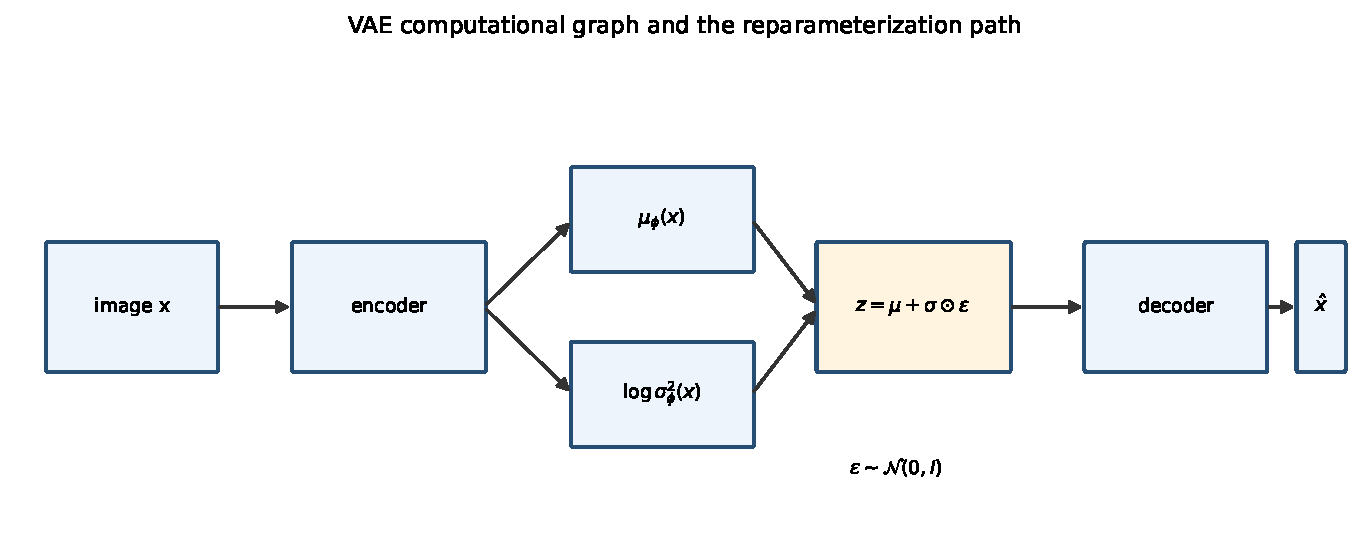
\includegraphics[width=0.96\textwidth]{fig12_04_vae_graph.pdf}
\caption{گراف محاسباتی VAE. بازپارامتردهی، منبع تصادف را از پارامترهای شبکه جدا می‌کند تا گرادیان pathwise قابل محاسبه باشد.}
\end{figure}

\subsection{بازپارامتردهی گاوسی}
اگر
\begin{equation}
 q_\phi(\vect z\mid\vect x)=\mathcal N(\vect\mu_\phi(\vect x),\diag(\vect\sigma_\phi^2(\vect x))),
\end{equation}
آنگاه نمونه را به صورت
\begin{equation}
 \vect\epsilon\sim\mathcal N(0,I),\qquad
 \vect z=\vect\mu_\phi(\vect x)+\vect\sigma_\phi(\vect x)\odot\vect\epsilon
\end{equation}
می‌نویسیم. اکنون تصادف در $\epsilon$ مستقل از پارامتر است و مشتق از مسیر تعیین‌گرای بعدی عبور می‌کند. برای تابع $h$،
\begin{equation}
 \nabla_\phi \E_{q_\phi(z\mid x)}h(z)
 =\E_{\epsilon}\nabla_\phi h(\mu_\phi+\sigma_\phi\odot\epsilon).
\end{equation}

\begin{figure}[H]
\centering
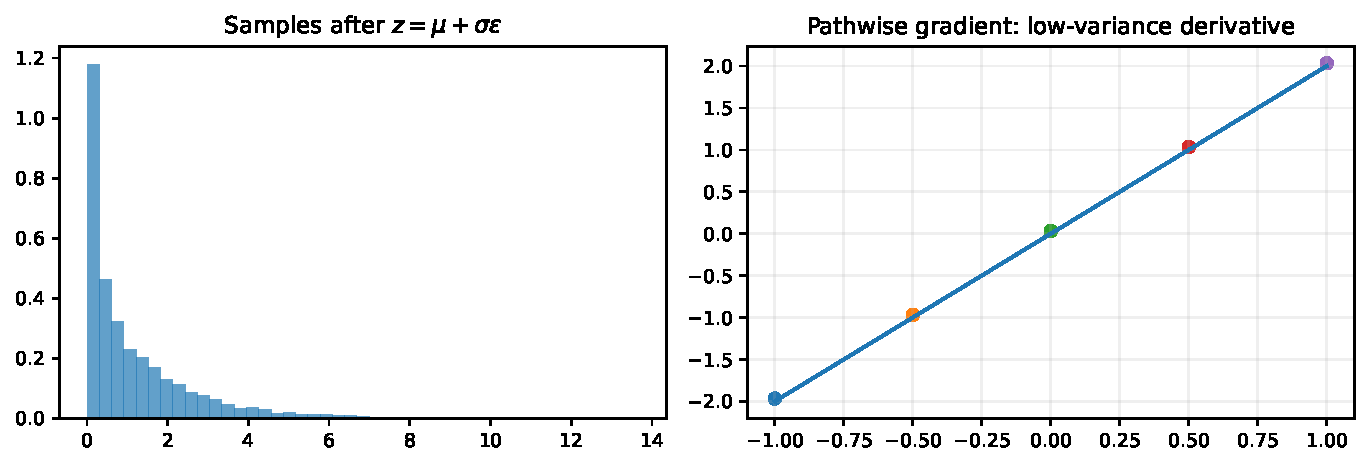
\includegraphics[width=0.94\textwidth]{fig12_06_reparameterization.pdf}
\caption{بازپارامتردهی گاوسی نمونه‌گیری را به یک تبدیل مشتق‌پذیر از نویز استاندارد تبدیل می‌کند.}
\end{figure}

\subsection{KL بسته برای گاوسی قطری}
برای prior استاندارد،
\begin{equation}
 \KL(q_\phi(z\mid x)\Vert\mathcal N(0,I))
 =\frac12\sum_{j=1}^{d_z}
 \left(\mu_j^2+\sigma_j^2-1-\log\sigma_j^2\right).
\end{equation}
در کد بهتر است شبکه $\log\sigma^2$ را خروجی دهد، آن را در بازه‌ای ایمن clamp کند و از
$\sigma=\exp(\tfrac12\log\sigma^2)$ استفاده شود.

\subsection{مدل مشاهده و معنای زیان بازسازی}
زیان بازسازی انتخابی دلخواه نیست؛ منفی log-likelihood مدل مشاهده است:
\begin{itemize}
\item Bernoulli برای داده دودویی: binary cross-entropy؛
\item Gaussian با واریانس ثابت: MSE تا ضریب و ثابت؛
\item Gaussian با واریانس آموختنی: جمله $\log\sigma^2$ نیز ضروری است؛
\item discretized logistic mixture برای پیکسل‌های گسسته رنگی؛
\item Laplace: زیان $\ell_1$؛
\item likelihood ادراکی: مدل آماری دقیق پیکسل نیست و باید با احتیاط تفسیر شود.
\end{itemize}

\subsection{تجزیه نرخ ـ اعوجاج}
نسخه $\beta$-VAE
\begin{equation}
 \mathcal L_\beta=\E_q[-\log p_\theta(x\mid z)]+\beta\KL(q(z\mid x)\Vert p(z))
\end{equation}
میان اعوجاج بازسازی و نرخ نهفته مبادله ایجاد می‌کند. افزایش $\beta$ معمولاً فشرده‌سازی و جداسازی عوامل را تقویت می‌کند ولی
جزئیات را کاهش می‌دهد. این تعبیر از برچسب مبهم «regularization بیشتر» دقیق‌تر است.

\begin{figure}[H]
\centering
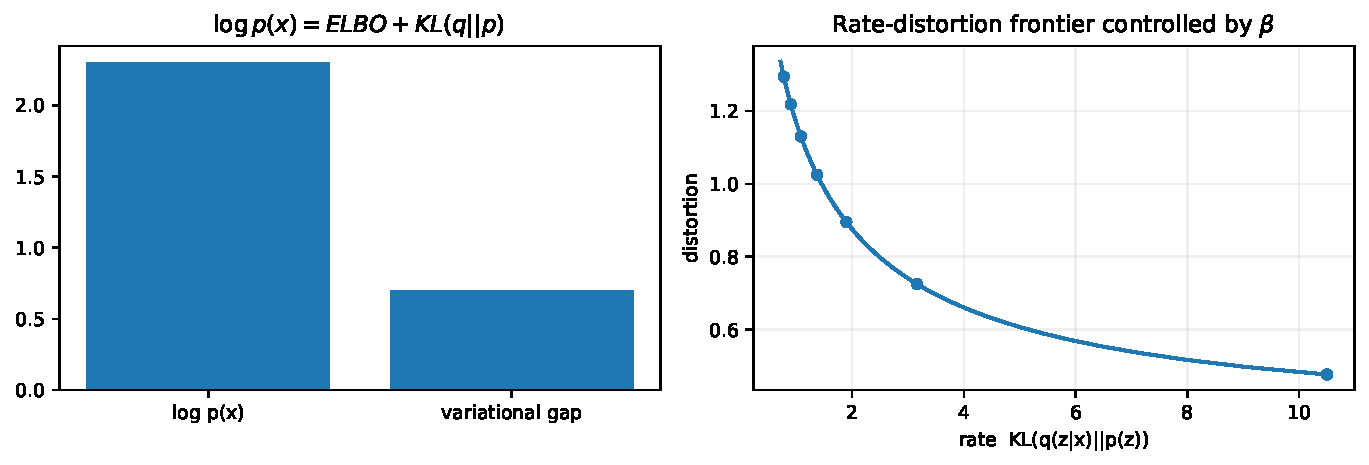
\includegraphics[width=0.96\textwidth]{fig12_05_elbo_rate_distortion.pdf}
\caption{هویت ELBO و جبهه نرخ ـ اعوجاج. یک VAE خوب لزوماً کمترین خطای بازسازی را ندارد؛ باید نرخ نهفته نیز کنترل شود.}
\end{figure}

\begin{algorithmbox}{الگوریتم ۱۲.۱ ـ آموزش یک VAE گاوسی}
برای هر minibatch $x$:
\begin{enumerate}
\item $\mu,\log\sigma^2\leftarrow E_\phi(x)$؛
\item $\epsilon\sim\mathcal N(0,I)$ و $z=\mu+\exp(\tfrac12\log\sigma^2)\odot\epsilon$؛
\item پارامترهای likelihood را با $D_\theta(z)$ بسازید؛
\item $L_{\rm rec}=-\log p_\theta(x\mid z)$ و $L_{\rm KL}$ را محاسبه کنید؛
\item $L=L_{\rm rec}+\beta L_{\rm KL}$؛
\item گرادیان، clipping اختیاری، سپس به‌روزرسانی مشترک $\theta,\phi$؛
\item جداگانه recon، KL هر بعد، active units و نمونه prior را ثبت کنید.
\end{enumerate}
\end{algorithmbox}

\begin{workshopbox}[VAE حداقلی]
فایل \lr{code/vae\_minimal.py} یک VAE کاملاً مستقل برای بردارهای دودویی دارد و ELBO را به بازسازی و KL تفکیک می‌کند.
\begin{latin}
\lstinputlisting[firstline=1,lastline=55]{code/vae_minimal.py}
\end{latin}
تمرین: likelihood Bernoulli را به Gaussian با واریانس آموختنی تبدیل کنید و بررسی کنید اگر جمله $\log\sigma$ حذف شود،
شبکه چگونه واریانس را بی‌قاعده افزایش می‌دهد.
\end{workshopbox}

\section{فروپاشی پسین و عیب‌یابی VAE}
فروپاشی پسین یعنی
\begin{equation}
 q_\phi(z\mid x)\approx p(z)
\end{equation}
برای تعداد زیادی از نمونه‌ها و ابعاد؛ در نتیجه $z$ اطلاعات اندکی درباره $x$ دارد و decoder قدرتمند تقریباً مستقل از نهفته عمل می‌کند.
این پدیده فقط «KL کوچک» نیست؛ باید همراه با وابستگی بازسازی به $z$، active units و mutual information بررسی شود.

\subsection{چرا رخ می‌دهد؟}
\begin{itemize}
\item decoder خودرگرسیو یا بسیار پرظرفیت بدون $z$ نیز می‌تواند داده را توضیح دهد؛
\item در ابتدای آموزش، کاهش سریع KL راه ساده‌تری از استفاده از نهفته است؛
\item وزن یا schedule نامناسب KL؛
\item mismatch میان prior ساده و posterior واقعی؛
\item بهینه‌سازی نامتوازن encoder و decoder.
\end{itemize}

\subsection{آزمون‌های تشخیصی}
\begin{enumerate}
\item KL کل و KL هر بعد؛
\item تعداد active unit با $\Var_x[\E(z_j\mid x)]>\tau$؛
\item بازسازی پس از shuffle کردن $z$؛
\item شکاف بین بازسازی با mean و sample؛
\item برآورد اطلاعات متقابل $I_q(x;z)$؛
\item prior sample در برابر posterior sample.
\end{enumerate}

\subsection{راهکارها}
KL annealing، cyclical annealing، free bits، capacity scheduling، weakening decoder، skip از $z$، prior سلسله‌مراتبی،
posterior غنی‌تر با flow و objectiveهای جایگزین از راهکارهای رایج‌اند. هیچ‌کدام تضمین عمومی نیست؛ باید اثر بر نرخ، اعوجاج و کیفیت نمونه گزارش شود.

\begin{figure}[H]
\centering
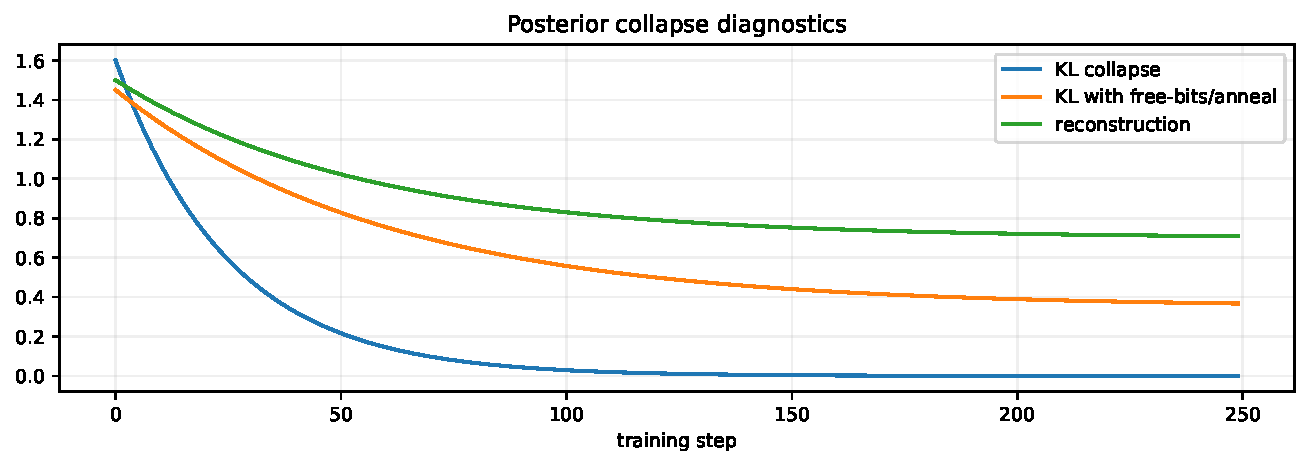
\includegraphics[width=0.94\textwidth]{fig12_07_posterior_collapse.pdf}
\caption{نمودار تشخیصی آموزشی. صفرشدن سریع KL در حالی که بازسازی بهبود می‌یابد می‌تواند نشانه نادیده‌گرفتن نهفته باشد.}
\end{figure}

\section{خانواده گسترده VAE}
\subsection{IWAE و کران چندنمونه‌ای}
با $K$ نمونه از $q$،
\begin{equation}
 \mathcal L_K=\E\left[\log\frac1K\sum_{k=1}^K
 \frac{p_\theta(x,z_k)}{q_\phi(z_k\mid x)}\right]
\end{equation}
کرانی است که با افزایش $K$ معمولاً تنگ‌تر می‌شود. با این حال، بهبود bound لزوماً به معنای نمایش بهتر encoder نیست و نسبت سیگنال به نویز گرادیان پارامترهای استنباط باید تحلیل شود.

\subsection{WAE و تطبیق posterior تجمعی}
posterior تجمعی
\begin{equation}
 q_\phi(z)=\int q_\phi(z\mid x)p_{\rm data}(x)dx
\end{equation}
است. WAE به‌جای مجبورکردن هر posterior شرطی به prior، توزیع تجمعی را با MMD یا منتقد خصمانه تطبیق می‌دهد:
\begin{equation}
 \E\,c(x,G(z))+\lambda D(q_\phi(z),p(z)).
\end{equation}
این تفاوت می‌تواند کدهای اطلاعاتی‌تر بسازد، ولی انتخاب $D$ و کرنل یا منتقد مهم است.

\subsection{مدل‌های سلسله‌مراتبی}
در مدل چندسطحی
\begin{equation}
 p(z_L)\prod_{\ell=1}^{L-1}p(z_\ell\mid z_{>\ell})p(x\mid z_{1:L}),
\end{equation}
متغیرهای سطح بالا ساختار کلی و سطوح پایین جزئیات را مدل می‌کنند. معماری‌هایی مانند \lr{NVAE} و \lr{VDVAE} برای
جلوگیری از بی‌استفاده‌شدن سطوح و کنترل ناپایداری، residual parameterization، normalizing flow در posterior و ترفندهای
بهینه‌سازی دارند. پیچیدگی این مدل‌ها نشان می‌دهد «افزودن چند latent» به‌تنهایی سلسله‌مراتب معنایی ایجاد نمی‌کند.

\subsection{VAE شرطی}
برای شرط $y$،
\begin{equation}
 p_\theta(x,z\mid y)=p_\theta(z\mid y)p_\theta(x\mid z,y),
\end{equation}
و encoder نیز $q_\phi(z\mid x,y)$ است. شرط می‌تواند کلاس، نقشه عمق، segmentation، متن یا تصویر دیگری باشد. باید روشن شود
کدام بخش شرط در prior، encoder و decoder تزریق می‌شود و آیا مدل از $z$ برای تنوع شرطی استفاده می‌کند یا خروجی تقریباً تعیین‌گراست.

\begin{figure}[H]
\centering
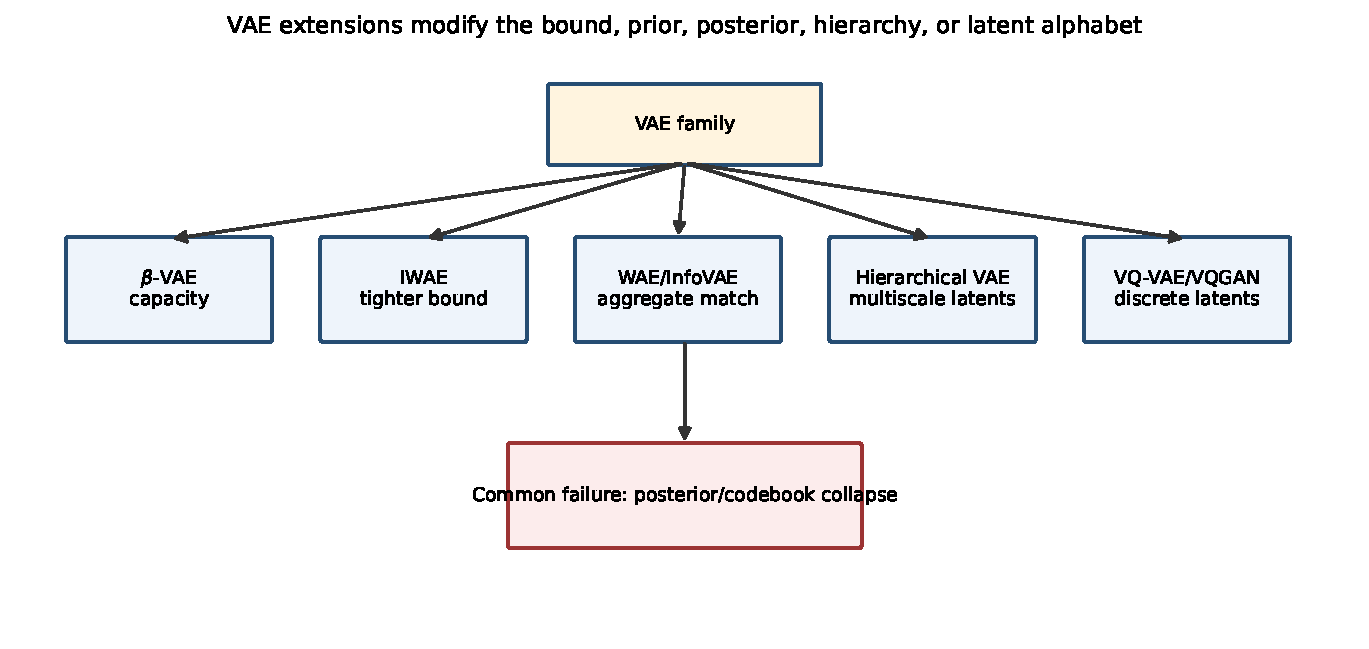
\includegraphics[width=0.98\textwidth]{fig12_09_vae_family.pdf}
\caption{نسخه‌های VAE یک مسئله واحد را حل نمی‌کنند؛ بعضی bound، بعضی prior/posterior، بعضی هندسه نهفته و بعضی الفبای نهفته را تغییر می‌دهند.}
\end{figure}

\section{VQ-VAE: متغیر نهفته گسسته و کد تصویری}
رمزگذار بردارهای $z_e(x)$ را تولید می‌کند و هر بردار به نزدیک‌ترین عضو codebook
$\{e_k\}_{k=1}^K$ نگاشت می‌شود:
\begin{equation}
 k^*=\argmin_k\norm{z_e(x)-e_k}_2^2,
 \qquad z_q(x)=e_{k^*}.
\end{equation}
quantization مشتق‌پذیر نیست. straight-through estimator در backward گرادیان decoder را تقریباً مستقیم به encoder می‌فرستد:
\begin{equation}
 z_{\rm st}=z_e+\sg(z_q-z_e).
\end{equation}
زیان رایج
\begin{equation}
 L=L_{\rm rec}+\norm{\sg(z_e)-e}^2+\beta\norm{z_e-\sg(e)}^2
\end{equation}
شامل به‌روزرسانی codebook و commitment است.

\subsection{Perplexity و codebook collapse}
اگر $p_k$ فراوانی استفاده از کد $k$ باشد،
\begin{equation}
 \operatorname{perplexity}=\exp\left(-\sum_k p_k\log p_k\right).
\end{equation}
perplexity پایین نسبت به $K$ می‌تواند نشان دهد بسیاری از کدها مرده‌اند؛ ولی perplexity بالا نیز کیفیت یا معنایی‌بودن کد را تضمین نمی‌کند.
باید reconstruction، rFID، entropy موضعی، occupancy، پایداری assignment و بعد مؤثر codebook با هم گزارش شوند.

\begin{figure}[H]
\centering
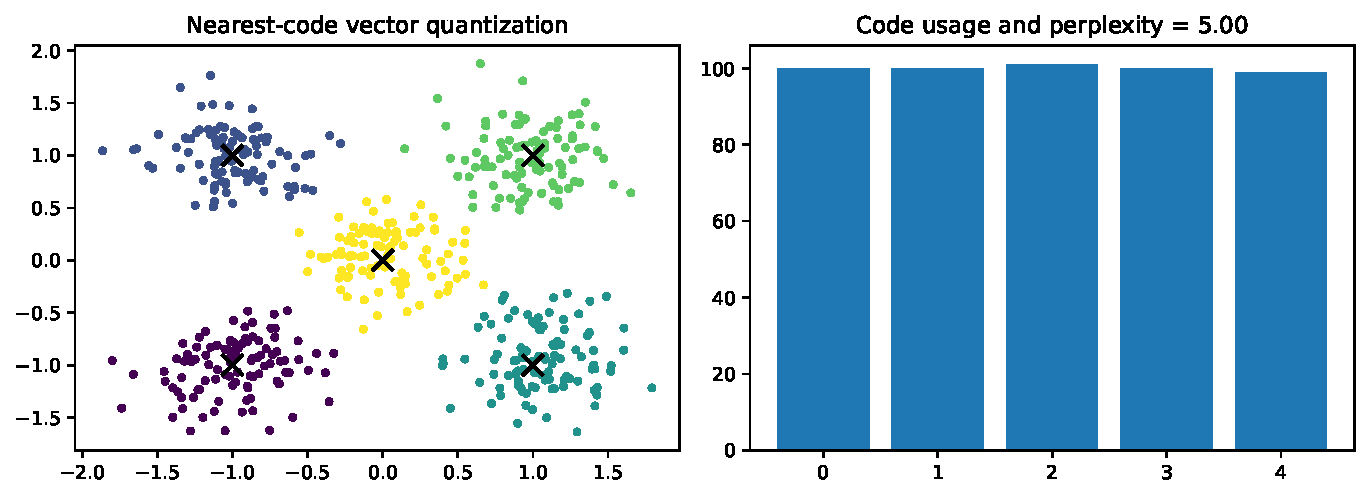
\includegraphics[width=0.94\textwidth]{fig12_08_vq_codebook.pdf}
\caption{کوانتیزه‌سازی برداری و سنجش استفاده از codebook. فروپاشی ممکن است به چند کد فعال یا زیر فضای بسیار کم‌بعد محدود شود.}
\end{figure}

\subsection{به‌روزرسانی EMA codebook}
به‌جای گرادیان مستقیم می‌توان شمارش و مجموع بردارهای هر کد را با میانگین نمایی به‌روزرسانی کرد. این روش شبیه k-means آنلاین است و
گاهی پایداری بیشتری دارد. initialization با k-means، reset کدهای مرده، residual quantization، product quantization و روش‌های
بدون codebook مانند finite scalar quantization نیز ابزارهای طراحی‌اند.

\subsection{VQGAN و حد بالای کیفیت tokenizer}
VQGAN بازسازی را با زیان ادراکی و منتقد patch ترکیب می‌کند تا latent grid فشرده ولی از نظر ادراکی دقیق بسازد. سپس یک Transformer
توزیع کدها را مدل می‌کند. این جداسازی دو خطا ایجاد می‌کند:
\begin{equation}
 \text{خطای نهایی}=\text{خطای tokenizer}+\text{خطای prior روی tokenها}.
\end{equation}
اگر tokenizer جزئیات را حذف کند، مدل مولد مرحله دوم قادر به بازیابی وفادار آن‌ها نیست؛ ممکن است صرفاً جزئیات plausible بسازد.

\begin{workshopbox}[VQ-VAE حداقلی]
فایل \lr{code/vq\_vae\_minimal.py} nearest-code، straight-through، commitment loss و perplexity را پیاده می‌کند.
\begin{latin}
\lstinputlisting[firstline=1,lastline=65]{code/vq_vae_minimal.py}
\end{latin}
آزمایش پیشنهادی: $K$، بعد code و $\beta$ را تغییر دهید و سه نمودار reconstruction، perplexity و effective rank codebook را هم‌زمان رسم کنید.
\end{workshopbox}

\section{GAN: یادگیری توزیع به‌وسیله بازی تمایز}
مدل اصلی GAN بازی زیر را تعریف می‌کند:
\begin{equation}
 \min_G\max_D V(D,G)=
 \E_{x\sim p_{\rm data}}\log D(x)
 +\E_{z\sim p(z)}\log(1-D(G(z))).
 \label{eq:gan-minimax}
\end{equation}
$D(x)$ احتمال واقعی‌بودن نیست مگر تحت فرض‌های دقیق و کالیبراسیون مناسب؛ در تحلیل نظریِ تمایزگر بهینه، یک نسبت چگالی است.

\begin{figure}[H]
\centering
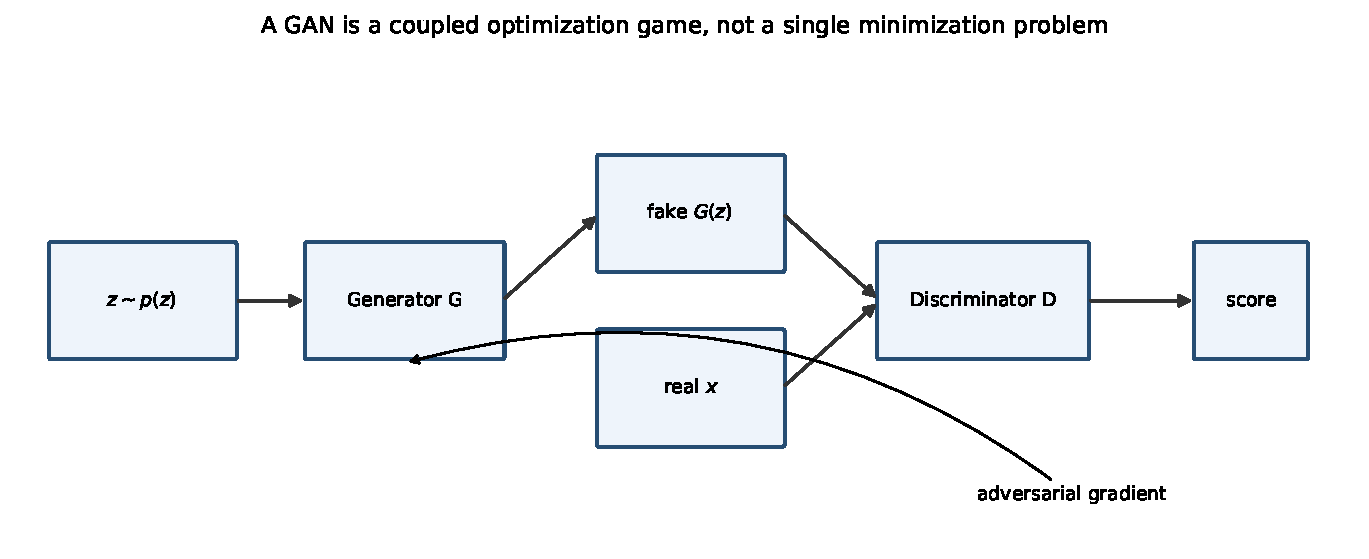
\includegraphics[width=0.96\textwidth]{fig12_10_gan_game.pdf}
\caption{حلقه GAN. تمایزگر تابع زیان داده‌محور برای مولد می‌سازد و مولد هم‌زمان توزیع ورودی تمایزگر را تغییر می‌دهد.}
\end{figure}

\subsection{استخراج تمایزگر بهینه}
برای $G$ ثابت، تابع هدف نقطه‌به‌نقطه
\begin{equation}
 p_{\rm data}(x)\log D(x)+p_g(x)\log(1-D(x))
\end{equation}
است. مشتق نسبت به $D(x)$ را صفر می‌کنیم:
\begin{equation}
 \frac{p_{\rm data}}{D}-\frac{p_g}{1-D}=0
 \quad\Longrightarrow\quad
 D^*(x)=\frac{p_{\rm data}(x)}{p_{\rm data}(x)+p_g(x)}.
\end{equation}
جایگذاری می‌دهد:
\begin{equation}
 V(D^*,G)=-\log4+2\JS(p_{\rm data}\Vert p_g).
\end{equation}
این نتیجه درباره تمایزگر بهینه و ظرفیت نامحدود است؛ آموزش عملی با شبکه محدود، minibatch و بهینه‌سازی ناتمام دقیقاً این واگرایی را کمینه نمی‌کند.

\begin{figure}[H]
\centering
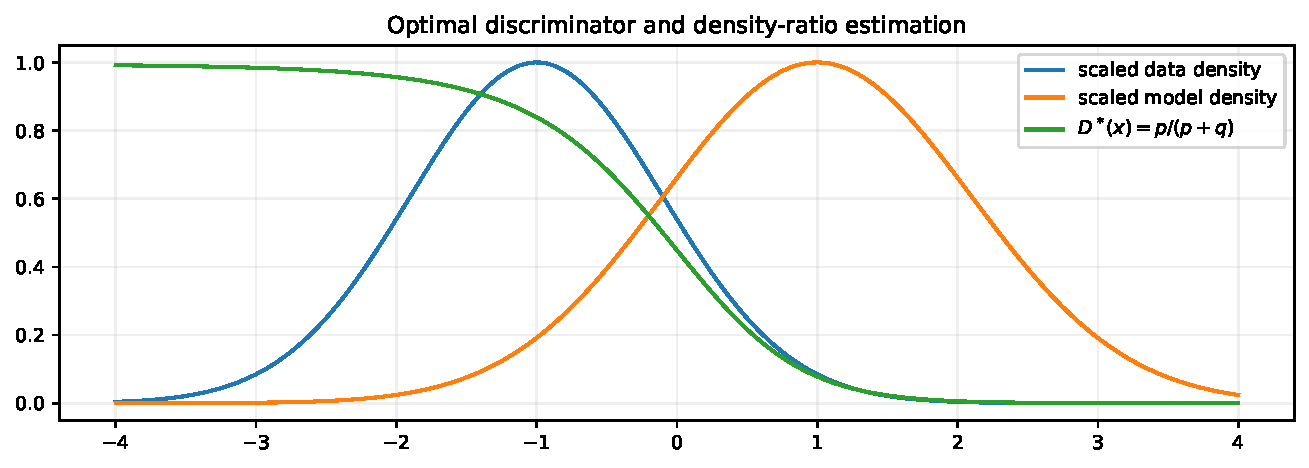
\includegraphics[width=0.93\textwidth]{fig12_11_optimal_discriminator.pdf}
\caption{تمایزگر بهینه نسبت چگالی را به یک احتمال لوجستیک تبدیل می‌کند. در نواحی فقط واقعی به یک و فقط مصنوعی به صفر میل می‌کند.}
\end{figure}

\subsection{زیان غیر اشباع مولد}
در نسخه minimax، هنگامی که $D(G(z))\approx0$، gradient از sigmoid ممکن است ضعیف باشد. زیان غیر اشباع
\begin{equation}
 L_G^{\rm NS}=-\E_z\log D(G(z))
\end{equation}
همان نقطه تعادل را هدف می‌گیرد ولی gradient قوی‌تری در ابتدای آموزش دارد. hinge loss نیز در مدل‌های تصویری رایج است:
\begin{align}
 L_D&=\E_x\max(0,1-D(x))+\E_z\max(0,1+D(G(z))),\\
 L_G&=-\E_zD(G(z)).
\end{align}

\section{چرا GAN ناپایدار است؟}
آموزش GAN کمینه‌سازی یک تابع ثابت نیست، بلکه یافتن تعادل یک بازی است. اگر پارامترها $\theta_G,\theta_D$ باشند، میدان گرادیان
\begin{equation}
 F(\theta)=\begin{bmatrix}\nabla_{\theta_G}L_G\\ \nabla_{\theta_D}L_D\end{bmatrix}
\end{equation}
می‌تواند مؤلفه دورانی داشته باشد. بنابراین loss ممکن است نوسان کند و کاهش یکنواخت انتظار درستی نیست.

\subsection{فروپاشی مد}
مولد ممکن است چندین $z$ را به یک یا چند مد محدود ببرد. علت‌ها شامل gradient مشابه، منتقد ناکافی، عدم تعادل سرعت یادگیری،
هدف mode-seeking و داده محدود است. تشخیص باید با coverage، precision/recall، occupancy کلاس، pairwise diversity، nearest-neighbor
و آزمون latent sensitivity انجام شود؛ تصویر خوب منتخب، collapse را رد نمی‌کند.

\begin{figure}[H]
\centering
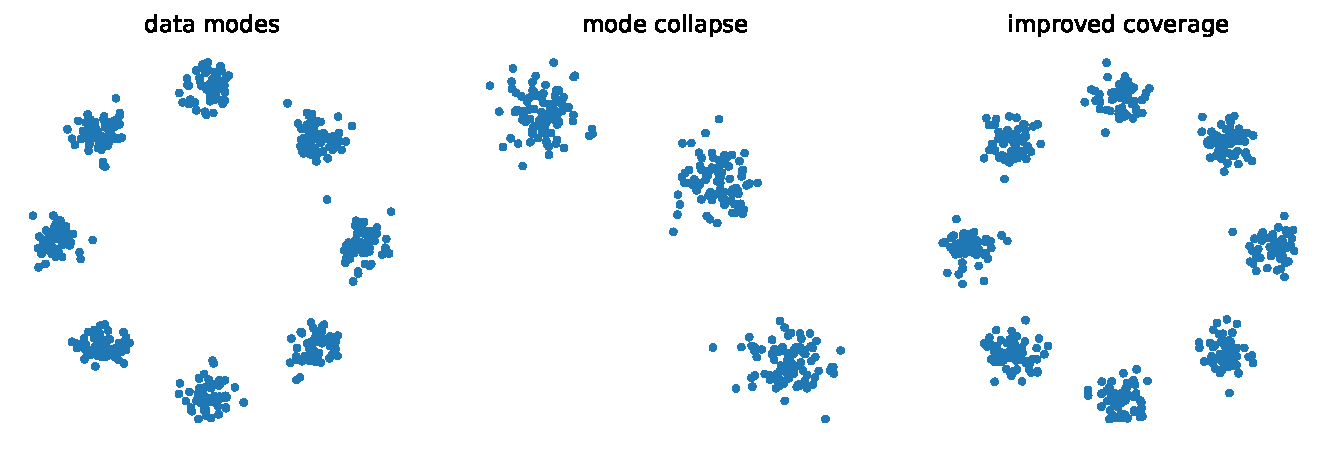
\includegraphics[width=0.96\textwidth]{fig12_12_mode_collapse.pdf}
\caption{نمایش دوبعدی فروپاشی مد. کیفیت موضعی نمونه‌ها ممکن است بالا باشد، ولی پوشش توزیع ناقص بماند.}
\end{figure}

\subsection{برتری بیش از حد تمایزگر}
تمایزگر بسیار قوی می‌تواند داده آموزش را حفظ کند و سطح تصمیم تیز بسازد؛ در نتیجه gradient مولد بدشرط می‌شود. تمایزگر بسیار ضعیف نیز
سیگنال مفیدی نمی‌دهد. نسبت تعداد updateها، ظرفیت، augmentation، regularization و نرخ یادگیری باید بر اساس تشخیص، نه قاعده ثابت، تنظیم شود.

\begin{figure}[H]
\centering
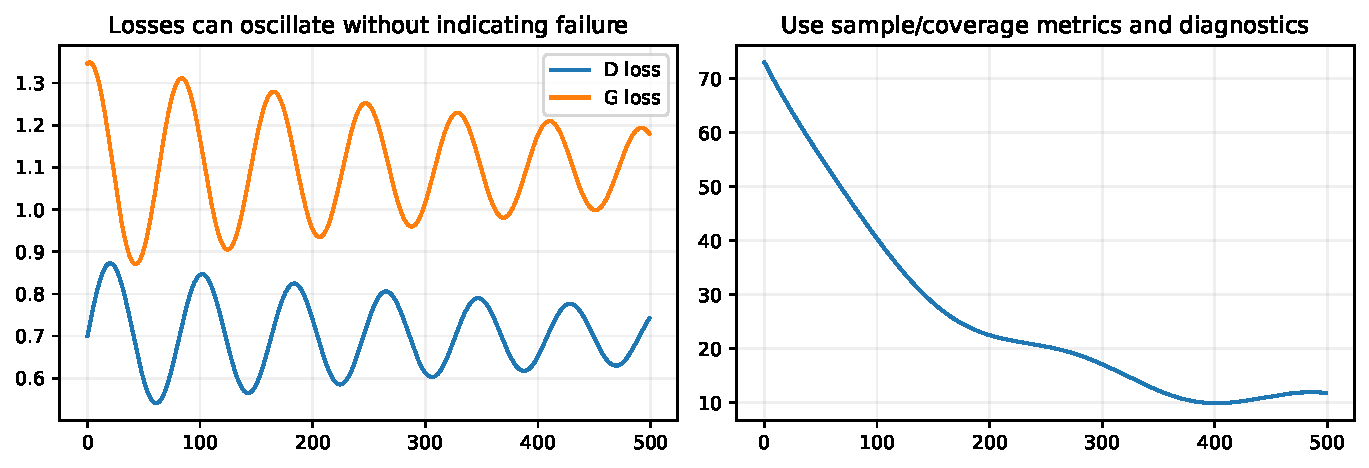
\includegraphics[width=0.94\textwidth]{fig12_14_gan_dynamics.pdf}
\caption{زیان‌های GAN به‌تنهایی معیار کیفیت نیستند. نمونه ثابت، معیار پوشش، norm گرادیان و FID/KID روی پروتکل ثابت لازم‌اند.}
\end{figure}

\section{WGAN و هندسه Lipschitz}
WGAN از دوگان Wasserstein استفاده می‌کند:
\begin{equation}
 \max_{\psi:\norm{f_\psi}_L\le1}
 \E_{x\sim p_{\rm data}}f_\psi(x)-\E_{z}f_\psi(G_\theta(z)).
\end{equation}
خروجی $f$ دیگر احتمال نیست و critic نامیده می‌شود. قید یک-Lipschitz بخش اصلی نظریه است.

\subsection{چرا weight clipping نامناسب است؟}
clipping فضای پارامتر را محدود می‌کند، نه مستقیماً ثابت Lipschitz تابع را. می‌تواند ظرفیت critic را کم و gradient را اشباع یا قطعه‌ای کند.

\subsection{Gradient penalty}
WGAN-GP روی نقاط میان داده واقعی و مصنوعی
\begin{equation}
 \hat x=\epsilon x+(1-\epsilon)\tilde x,
 \qquad \epsilon\sim U(0,1)
\end{equation}
جریمه
\begin{equation}
 \lambda\E_{\hat x}\left(\norm{\nabla_{\hat x}f(\hat x)}_2-1\right)^2
\end{equation}
را اضافه می‌کند. این قید تنها روی مسیرهای نمونه‌برداری‌شده اعمال می‌شود و تضمین global Lipschitz کامل نیست.

\begin{figure}[H]
\centering
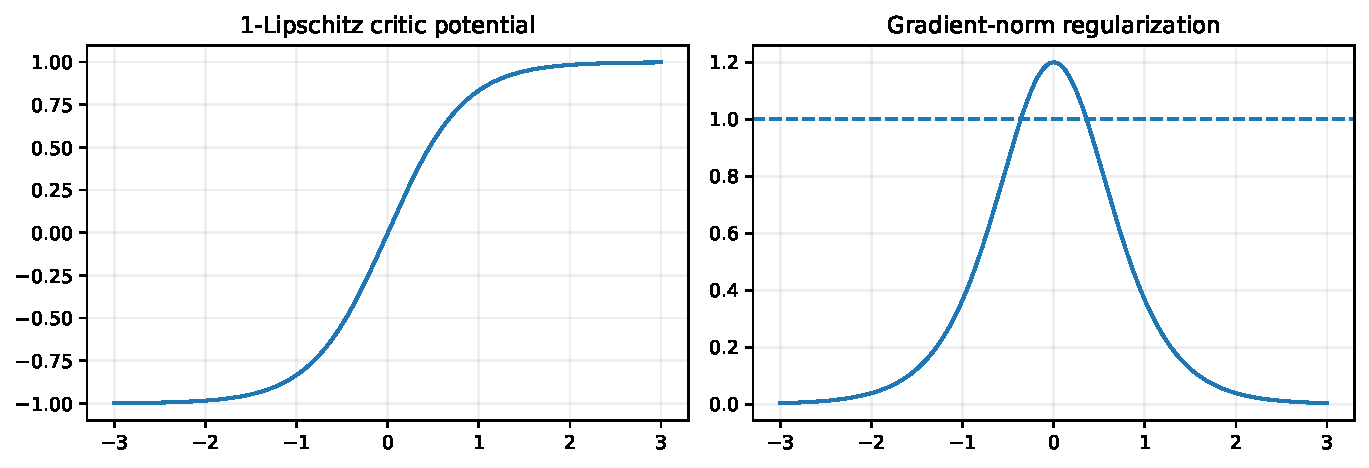
\includegraphics[width=0.94\textwidth]{fig12_13_wgan_lipschitz.pdf}
\caption{critic هموار و جریمه norm گرادیان. هدف، فراهم‌کردن شیب معنادار میان تکیه‌گاه‌های داده و مدل است.}
\end{figure}

\subsection{Spectral normalization}
برای لایه خطی $h=W x$، ثابت Lipschitz با $\sigma_{\max}(W)$ کران می‌شود. spectral normalization از
\begin{equation}
 \bar W=\frac{W}{\sigma_{\max}(W)}
\end{equation}
استفاده می‌کند و بزرگ‌ترین مقدار منفرد را با power iteration تقریب می‌زند. حاصل ضرب کران لایه‌ها یک کران شبکه می‌دهد، هرچند شل است.

\subsection{R1، lazy regularization و TTUR}
جریمه R1
\begin{equation}
 \frac\gamma2\E_{x\sim p_{\rm data}}\norm{\nabla_xD(x)}^2
\end{equation}
تمایزگر را نزدیک داده واقعی هموار می‌کند. در StyleGAN این جریمه ممکن است هر چند گام یک‌بار اعمال و ضریب آن برای حفظ امید تنظیم شود.
TTUR نرخ‌های یادگیری متفاوت برای دو بازیکن دارد و EMA وزن‌های مولد برای نمونه‌گیری پایدار استفاده می‌شود.

\begin{algorithmbox}{الگوریتم ۱۲.۲ ـ یک گام WGAN-GP}
\begin{enumerate}
\item $x\sim p_{\rm data}$، $z\sim p(z)$ و $\tilde x=G(z)$؛
\item critic loss: $\E f(\tilde x)-\E f(x)+\lambda GP$؛
\item چند update critic برای هر update مولد، در صورت نیاز؛
\item مولد: $L_G=-\E f(G(z))$؛
\item norm گرادیان، score واقعی/مصنوعی، coverage و نمونه‌های ثابت ثبت شوند؛
\item EMA مولد فقط برای ارزیابی نگهداری شود و وزن online نیز ذخیره گردد.
\end{enumerate}
\end{algorithmbox}

\begin{workshopbox}[GAN و WGAN-GP روی مخلوط گاوسی]
\begin{latin}
\lstinputlisting[firstline=1,lastline=70]{code/gan_minimal.py}
\end{latin}
فایل \lr{code/wgan\_gp\_minimal.py} جریمه گرادیان را با \lr{autograd} محاسبه می‌کند. روی هشت مد دوبعدی، occupancy هر مد را
در طول آموزش رسم کنید و نشان دهید loss تنها برای تشخیص collapse کافی نیست.
\end{workshopbox}

\section{معماری‌های مهم GAN}
\subsection{DCGAN: قرارداد معماری پایه}
DCGAN استفاده منظم از \lr{convolution} با \lr{stride}، \lr{batch normalization}، \lr{ReLU} در مولد و \lr{LeakyReLU} در تمایزگر را تثبیت کرد. اهمیت آن
بیشتر از یک مدل تاریخی است؛ یک \lr{baseline} شفاف برای بررسی تابع هدف و خط لوله داده است. با این حال، \lr{transposed convolution} می‌تواند
الگوی شطرنجی بسازد و \lr{BatchNorm} در دسته‌های کوچک ناپایدار است.

\subsection{شرطی‌سازی و projection discriminator}
در GAN شرطی، $G(z,y)$ و $D(x,y)$ داریم. projection discriminator score را به صورت
\begin{equation}
 D(x,y)=u^\top h(x)+e(y)^\top h(x)
\end{equation}
می‌سازد و سازگاری ویژگی تصویر با embedding کلاس را مستقیماً می‌سنجد. ACGAN یک سر طبقه‌بندی نیز اضافه می‌کند، ولی ممکن است
کیفیت و تنوع را با هدف طبقه‌بندی درهم بیامیزد.

\subsection{pix2pix و PatchGAN}
برای داده زوج‌شده $(x,y)$،
\begin{equation}
 L=L_{\rm cGAN}(G,D)+\lambda\norm{y-G(x)}_1.
\end{equation}
منتقد patch به‌جای یک score کلی، واقعی‌بودن وصله‌ها را می‌سنجد؛ بنابراین جزئیات بافت را تقویت می‌کند ولی سازگاری جهانی را تضمین نمی‌کند.

\subsection{CycleGAN و عدم شناساپذیری}
برای داده بدون زوج، دو نگاشت $G:X\to Y$ و $F:Y\to X$ و زیان
\begin{equation}
 L_{\rm cyc}=\E_x\norm{F(G(x))-x}_1+\E_y\norm{G(F(y))-y}_1
\end{equation}
اضافه می‌شود. cycle consistency نگاشت را محدود می‌کند ولی correspondence معنایی یکتا نمی‌سازد؛ نگاشت‌های اطلاعات‌پنهان و تغییرات نامطلوب
ممکن‌اند. برای کاربرد پزشکی یا علمی، حفظ ساختار باید با قیدهای مستقل آزمون شود.

\subsection{BigGAN و مقیاس}
BigGAN نشان داد batch بزرگ، مدل بزرگ، class embedding، spectral normalization و truncation می‌توانند کیفیت شرطی را افزایش دهند.
truncation $z$ را به ناحیه پرچگالی prior محدود می‌کند و معمولاً precision را به بهای recall افزایش می‌دهد؛ بنابراین یک knob ارزیابی است، نه بهبود رایگان.

\section{خانواده StyleGAN و هندسه فضای نهفته}
StyleGAN نگاشت $z\mapsto w$ را از synthesis جدا و style را در هر مقیاس تزریق می‌کند. فضای‌های متداول:
\begin{itemize}
\item $\mathcal Z$: prior ورودی؛
\item $\mathcal W$: خروجی mapping network؛
\item $\mathcal W^+$: style مستقل برای هر لایه؛
\item StyleSpace: پارامترهای modulation لایه‌ها.
\end{itemize}
افزایش آزادی inversion را آسان‌تر ولی prior مولد را ضعیف‌تر می‌کند؛ projection دقیق در $W^+$ الزاماً نمونه طبیعی روی منیفلد مدل نیست.

\subsection{Modulation و demodulation در StyleGAN2}
وزن convolution برای نمونه با style $s_i$ مدوله می‌شود:
\begin{equation}
 w'_{ijk}=s_iw_{ijk},
\end{equation}
سپس برای کنترل مقیاس خروجی demodulate می‌شود:
\begin{equation}
 w''_{ijk}=\frac{w'_{ijk}}{\sqrt{\sum_{i,k}(w'_{ijk})^2+\epsilon}}.
\end{equation}
path-length regularization تلاش می‌کند تغییر هم‌اندازه در $w$ اثر قابل پیش‌بینی‌تری در تصویر داشته باشد.

\subsection{StyleGAN3 و حذف alias}
StyleGAN3 سیگنال‌های داخلی را نمونه‌هایی از میدان پیوسته در نظر می‌گیرد و resampling فیلترشده و عملیات equivariant را برای جلوگیری از
texture sticking به‌کار می‌برد. این دیدگاه، فصل نمونه‌برداری و aliasing را مستقیماً به طراحی مولد عمیق پیوند می‌دهد.

\begin{figure}[H]
\centering
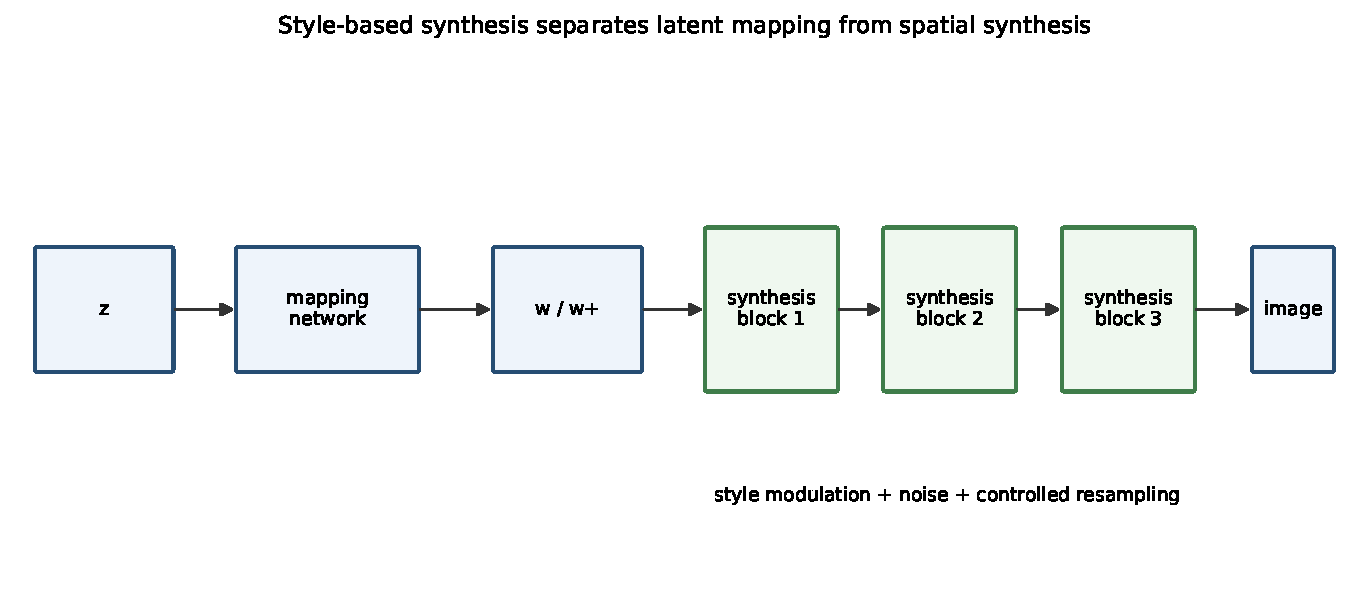
\includegraphics[width=0.96\textwidth]{fig12_15_stylegan.pdf}
\caption{ساختار مفهومی StyleGAN. mapping network هندسه prior را تغییر می‌دهد و styleهای چندمقیاسی synthesis را کنترل می‌کنند.}
\end{figure}

\subsection{Inversion و ویرایش}
Inversion می‌تواند با بهینه‌سازی latent، encoder یا روش هیبرید انجام شود:
\begin{equation}
 w^*=\argmin_w \ell_{\rm pix}(G(w),x)+\lambda\ell_{\rm perc}(G(w),x)+R(w).
\end{equation}
سه معیار جدا لازم است: fidelity بازسازی، editability و قرارداشتن در ناحیه طبیعی latent. بهبود یکی ممکن است دیگری را تضعیف کند.

\section{مدل‌های خودرگرسیو: چگالی دقیق با قاعده زنجیره}
برای ترتیب ثابت مؤلفه‌ها،
\begin{equation}
 p(x)=\prod_{i=1}^{D}p(x_i\mid x_{<i}).
\end{equation}
در آموزش همه conditionalها با teacher forcing به‌طور موازی محاسبه می‌شوند، اما نمونه‌گیری معمولاً ترتیبی است.

\begin{figure}[H]
\centering
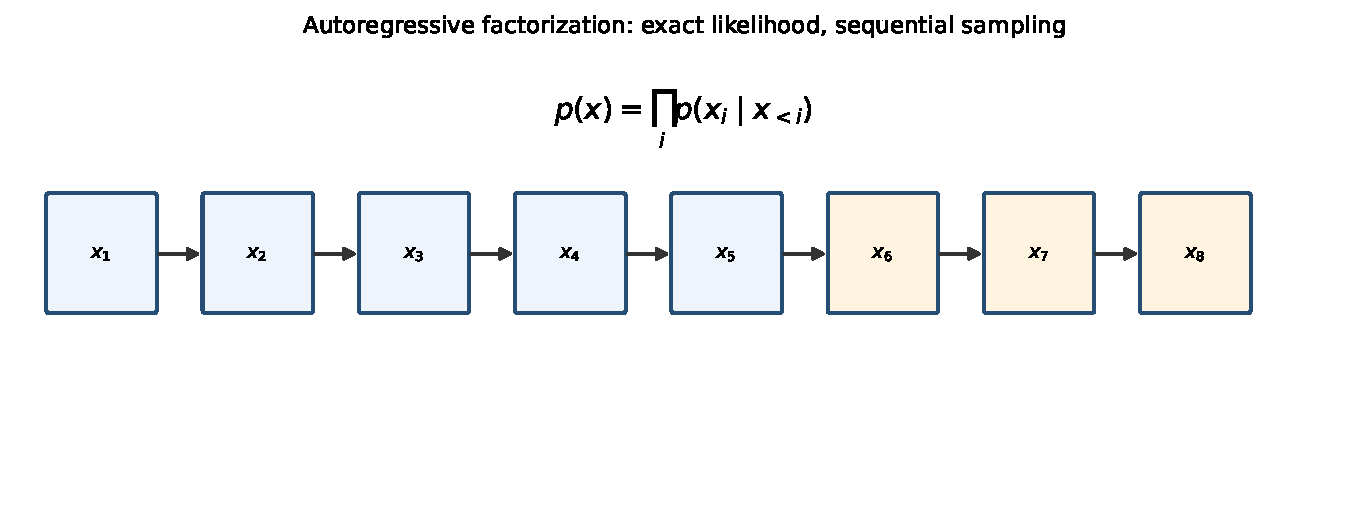
\includegraphics[width=0.95\textwidth]{fig12_16_autoregressive_chain.pdf}
\caption{قاعده زنجیره، likelihood دقیق را به conditionalهای ساده‌تر می‌شکند؛ هزینه آن ترتیب مصنوعی و sampling متوالی است.}
\end{figure}

\subsection{PixelRNN، PixelCNN و masked convolution}
mask باید تضمین کند خروجی مکان $i$ به $x_i$ یا آینده دسترسی ندارد. ماسک نوع A در لایه نخست مرکز را نیز حذف می‌کند و نوع B در لایه‌های بعدی
مرکز feature قبلی را مجاز می‌داند. خطای یک پیکسل در mask باعث leakage و درست‌نمایی جعلی می‌شود.

\begin{figure}[H]
\centering
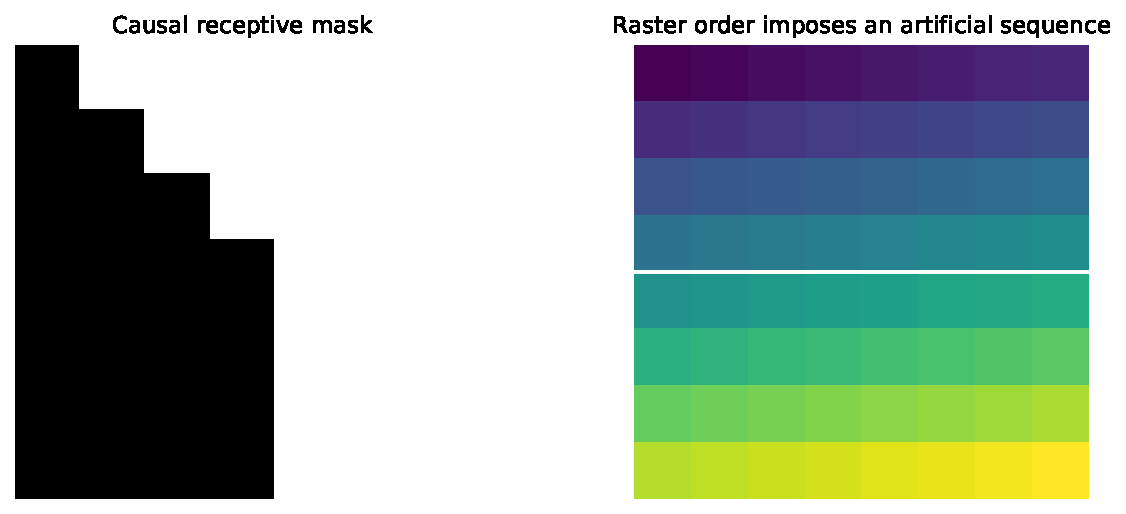
\includegraphics[width=0.92\textwidth]{fig12_17_masked_convolution.pdf}
\caption{mask علّی و ترتیب raster. ترتیب پیکسل یک ساختار فیزیکی ذاتی تصویر نیست و روی دشواری مدل اثر می‌گذارد.}
\end{figure}

\subsection{likelihood پیکسل رنگی}
مدل‌کردن هر مقدار ۸بیتی با softmax 256تایی ممکن است وابستگی کانال‌ها را نادیده بگیرد. discretized mixture of logistics جرم بازه کوانتیزه را
از اختلاف CDF محاسبه می‌کند و پارامترهای mixture، mean و scale را می‌آموزد. گزارش bits/dim باید دقیقاً با قرارداد dequantization و channel ordering همراه باشد.

\begin{workshopbox}[آزمون علّیت PixelCNN]
فایل \lr{code/pixelcnn\_mask.py} یک masked convolution آموزشی دارد. آزمون همراه آخرین پیکسل را تغییر می‌دهد و بررسی می‌کند logits مکان‌های قبلی تغییر نکنند.
\begin{latin}
\lstinputlisting[firstline=1,lastline=50]{code/pixelcnn_mask.py}
\end{latin}
این آزمون unit test مهم‌تری از مشاهده ظاهری نمونه‌هاست.
\end{workshopbox}

\section{از پیکسل به توکن: مولدهای تصویری خودرگرسیو جدید}
نمونه‌گیری پیکسلی برای تصویر بزرگ بسیار طولانی است. راهکار غالب، آموختن tokenizer و مدل‌کردن دنباله کدهاست:
\begin{equation}
 x\xrightarrow{E,Q} c_{1:N}\xrightarrow{p_\psi(c)}\hat c_{1:N}\xrightarrow{D}\hat x.
\end{equation}

\begin{figure}[H]
\centering
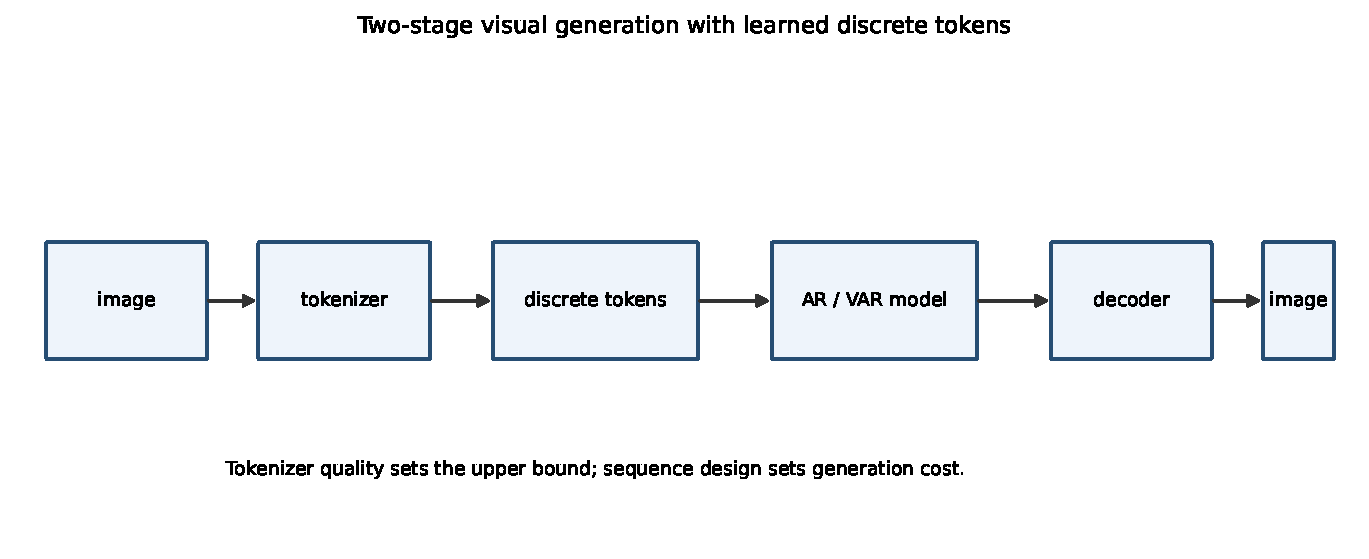
\includegraphics[width=0.96\textwidth]{fig12_18_token_ar.pdf}
\caption{مولد دومرحله‌ای. کیفیت tokenizer حد بالای وفاداری و تعداد/ترتیب token هزینه prior را تعیین می‌کند.}
\end{figure}

\subsection{VQGAN + Transformer}
کاهش تصویر به latent grid امکان مدل‌کردن ترکیب‌های دوربرد با Transformer را فراهم می‌کند. sliding attention برای رزولوشن بزرگ استفاده می‌شود.
در وظایف شرطی، tokenهای کلاس، متن، segmentation یا edge به دنباله افزوده می‌شوند.

\subsection{MaskGIT و decoding موازی تکراری}
به‌جای ترتیب چپ‌به‌راست، مدل tokenهای mask‌شده را پیش‌بینی می‌کند و در چند دور، مطمئن‌ترین tokenها را ثابت می‌سازد. این روش sampling را از $N$ گام
به تعداد دورهای کم کاهش می‌دهد، ولی conditional independence تقریبی و schedule mask مهم‌اند.

\subsection{LlamaGen و next-token prediction}
LlamaGen نشان می‌دهد یک Transformer علّی استاندارد روی tokenهای تصویری، با tokenizer و scaling مناسب، می‌تواند مولد رقابتی باشد. مزیت مهندسی آن
استفاده از زیرساخت serving مدل‌های زبانی است؛ محدودیت اصلی طول دنباله، خطای تجمعی و ترتیب raster است.

\subsection{VAR و next-scale prediction}
VAR به‌جای token بعدی، نقشه token مقیاس بعدی را از coarse به fine پیش‌بینی می‌کند:
\begin{equation}
 p(r_1,\ldots,r_S)=\prod_{s=1}^S p(r_s\mid r_{<s}).
\end{equation}
این ترتیب با ساختار چندمقیاسی تصویر سازگارتر و تعداد مراحل کمتر است. با این حال، ادعای برتری باید روی tokenizer، داده، compute و معیار یکسان سنجیده شود.

\subsection{توکن‌های یک‌بعدی فشرده}
TiTok تصویر را به دنباله کوتاه 1D تبدیل می‌کند. فشردگی بسیار بالا هزینه مولد را کاهش می‌دهد، اما فشار بیشتری به decoder و semantic compression وارد می‌کند.
پژوهش‌های ۲۰۲۵--۲۰۲۶ به token length تطبیقی، tokenهای مبتنی بر foundation model و جلوگیری از dimensional collapse codebook پرداخته‌اند.

\begin{keybox}[اصل مهندسی مولد توکنی]
هر نتیجه generation باید همراه با نتیجه مستقل tokenizer گزارش شود: reconstruction FID، LPIPS/PSNR، استفاده codebook، طول توکن، سرعت encoder/decoder و
حداکثر رزولوشن. در غیر این صورت معلوم نیست بهبود از prior است یا tokenizer.
\end{keybox}

\section{جریان‌های نرمال‌ساز: چگالی دقیق و نگاشت وارون‌پذیر}
اگر $f_\theta:x\mapsto z$ دوسویی و مشتق‌پذیر باشد،
\begin{equation}
 \log p_X(x)=\log p_Z(f_\theta(x))+
 \log\left|\det\frac{\partial f_\theta(x)}{\partial x}\right|.
 \label{eq:change-vars}
\end{equation}
نمونه‌گیری با $z\sim p_Z$ و $x=f_\theta^{-1}(z)$ انجام می‌شود. چالش، ساخت تبدیل بیانگر با determinant ژاکوبین ارزان است.

\subsection{Affine coupling در RealNVP}
$x=(x_a,x_b)$ را تقسیم کنید:
\begin{align}
 y_a&=x_a,\\
 y_b&=x_b\odot\exp s(x_a)+t(x_a).
\end{align}
ژاکوبین مثلثی است و
\begin{equation}
 \log|\det J|=\sum_j s_j(x_a).
\end{equation}
وارون نیز مستقیم است. نیمی از متغیرها در هر لایه ثابت می‌مانند؛ permutation یا invertible convolution برای اختلاط لازم است.

\begin{figure}[H]
\centering
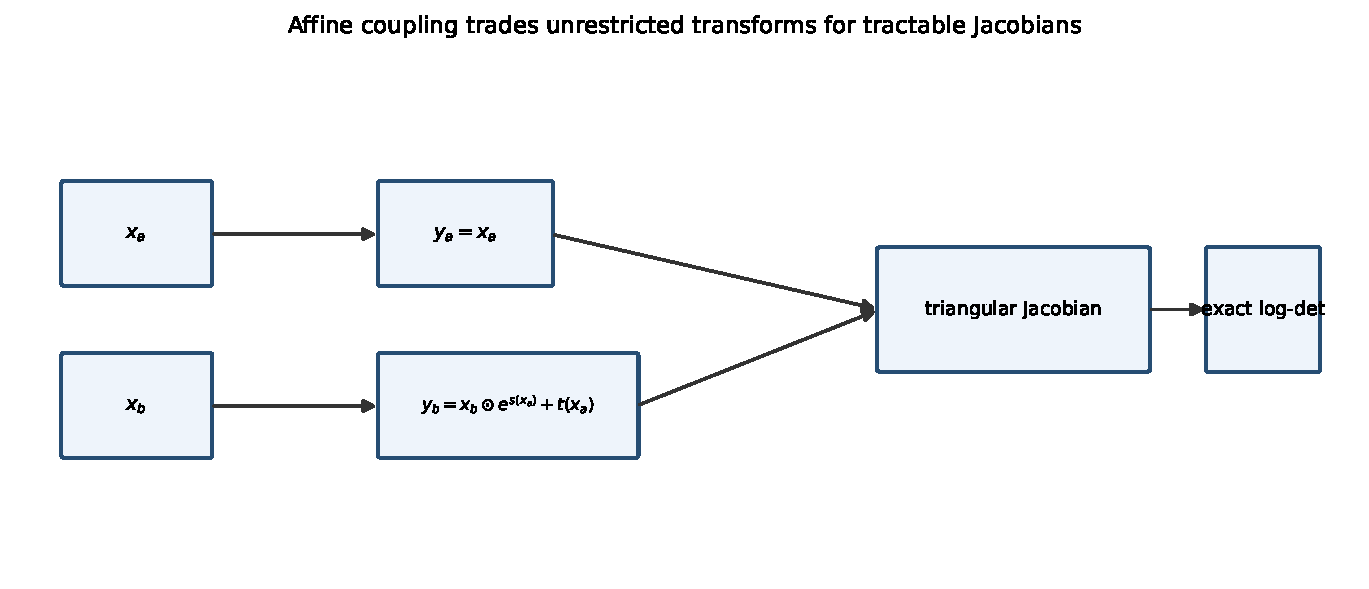
\includegraphics[width=0.95\textwidth]{fig12_19_flow_coupling.pdf}
\caption{coupling وارون‌پذیر. ساختار مثلثی ژاکوبین محاسبه log-determinant را ارزان می‌کند.}
\end{figure}

\subsection{Glow}
Glow سه جزء را تکرار می‌کند: ActNorm، convolution وارون‌پذیر $1\times1$ و affine coupling. ActNorm آمار اولیه داده را برای تنظیم bias/scale استفاده می‌کند؛
convolution وارون‌پذیر permutation آموختنی کانال‌هاست. معماری multi-scale بخشی از متغیرها را در سطوح مختلف factor-out می‌کند.

\subsection{MAF و IAF}
MAF محاسبه چگالی را موازی و نمونه‌گیری را ترتیبی می‌کند؛ IAF برعکس، نمونه‌گیری موازی و محاسبه density معکوس را مناسب‌تر برای posterior واریاسیونی می‌سازد.
انتخاب جهت باید با وظیفه inference یا generation هماهنگ باشد.

\subsection{Dequantization}
پیکسل گسسته را نمی‌توان بی‌واسطه با چگالی پیوسته مقایسه کرد. uniform dequantization
\begin{equation}
 y=x+u,\quad u\sim U[0,1)
\end{equation}
یک bound روی جرم گسسته می‌سازد. variational dequantization توزیع نویز شرطی را می‌آموزد. bits/dim بدون ذکر روش dequantization قابل مقایسه نیست.

\begin{workshopbox}[RealNVP دوبعدی و آزمون وارون]
\begin{latin}
\lstinputlisting[firstline=1,lastline=75]{code/realnvp_2d.py}
\end{latin}
آزمون اصلی باید $\max\abs{x-f^{-1}(f(x))}$ را نزدیک دقت ماشین نشان دهد. سپس log-det تحلیلی را با determinant عددی ژاکوبین در بعد کوچک مقایسه کنید.
\end{workshopbox}

\section{جریان‌های پیوسته و Flow Matching}
در continuous normalizing flow، حالت از ODE پیروی می‌کند:
\begin{equation}
 \frac{d x_t}{dt}=v_\theta(x_t,t).
\end{equation}
تغییر log-density با معادله آنی
\begin{equation}
 \frac{d}{dt}\log p_t(x_t)=-\trace\left(\frac{\partial v_\theta}{\partial x_t}\right)
\end{equation}
داده می‌شود. محاسبه trace در بعد بالا با Hutchinson تقریب زده می‌شود. آموزش CNF مبتنی بر likelihood ممکن است حل ODE در حلقه آموزش بخواهد.

Flow Matching میدان سرعت یک مسیر احتمال انتخابی را با regression می‌آموزد، بدون حل ODE در هر گام آموزش. در مسیر خطی ساده
\begin{equation}
 x_t=(1-t)x_0+tx_1,\qquad u_t=x_1-x_0,
\end{equation}
و هدف
\begin{equation}
 \E\norm{v_\theta(x_t,t)-u_t}^2
\end{equation}
است. مسیرهای انتقال بهینه می‌توانند trajectory مستقیم‌تر و sampling آسان‌تر بسازند. این بخش پلی مستقیم به فصل آینده diffusion و مدل‌های transport است.

\begin{figure}[H]
\centering
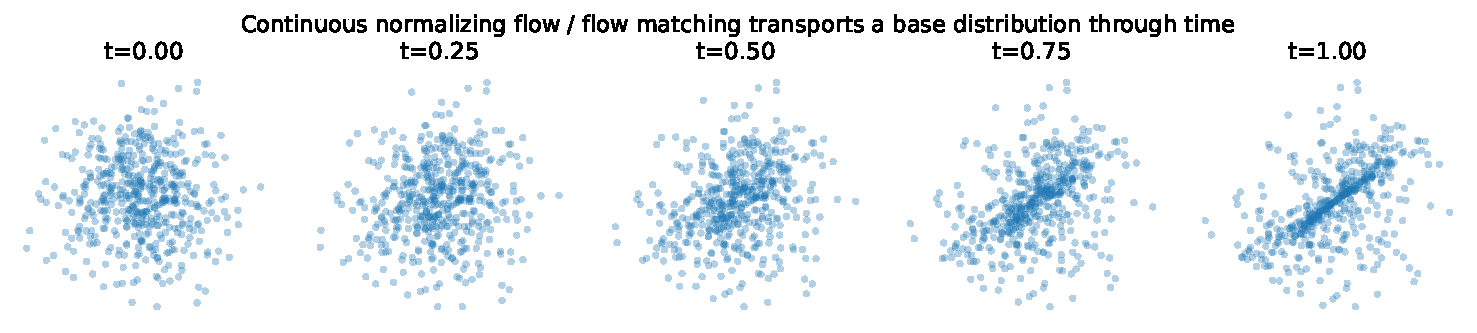
\includegraphics[width=0.98\textwidth]{fig12_20_continuous_flow.pdf}
\caption{انتقال پیوسته توزیع. مسیر احتمال و میدان سرعت دو شیء جدا هستند و انتخاب coupling روی دشواری regression اثر دارد.}
\end{figure}

\begin{workshopbox}[Flow Matching دوبعدی]
فایل \lr{code/flow\_matching\_2d.py} یک میدان سرعت را روی interpolation میان Gaussian و هشت مد آموزش می‌دهد. برای sampling، ODE را با Euler و RK4 حل و اثر تعداد گام را بر coverage اندازه‌گیری کنید.
\end{workshopbox}

\section{مدل‌های انرژی‌محور}
مدل انرژی
\begin{equation}
 p_\theta(x)=\frac{\exp[-E_\theta(x)]}{Z_\theta},
 \qquad Z_\theta=\int\exp[-E_\theta(x)]dx
\end{equation}
چگالی را تا ثابت نرمال‌سازی تعریف می‌کند. gradient درست‌نمایی
\begin{equation}
 \nabla_\theta\log p_\theta(x)=
 -\nabla_\theta E_\theta(x)
 +\E_{x'\sim p_\theta}\nabla_\theta E_\theta(x')
\end{equation}
دو فاز دارد: کاهش انرژی داده و افزایش انرژی نمونه مدل. فاز دوم به sampling از مدل نیاز دارد و دشوار است.

\begin{figure}[H]
\centering
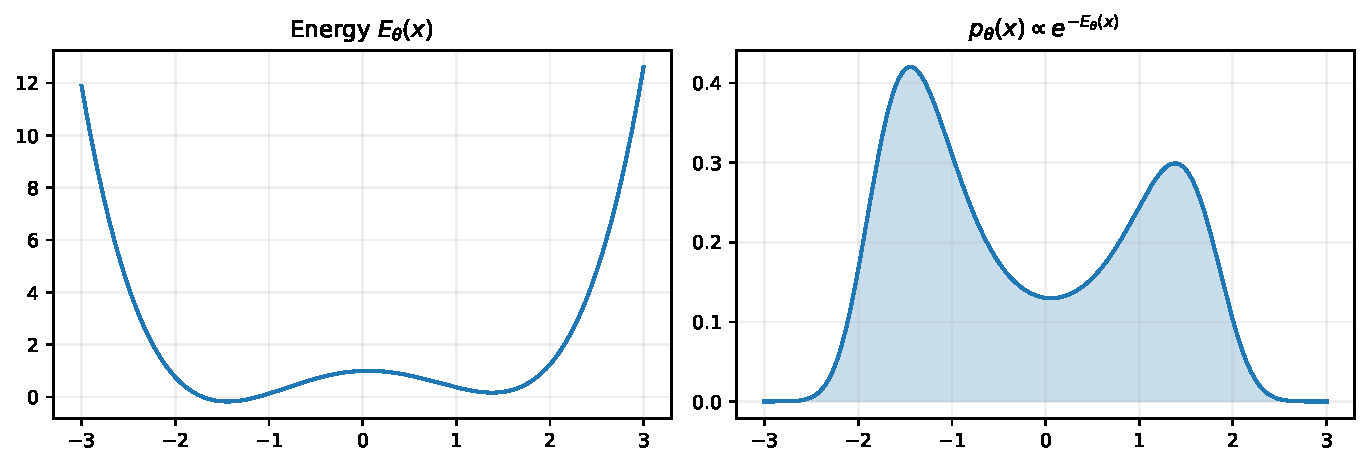
\includegraphics[width=0.93\textwidth]{fig12_21_energy_model.pdf}
\caption{مدل انرژی‌محور: چگالی بالا در دره‌های انرژی است، اما ثابت نرمال‌سازی و نمونه‌گیری از کل منظره دشوارند.}
\end{figure}

\subsection{Langevin dynamics}
نمونه‌گیری تقریبی با
\begin{equation}
 x_{k+1}=x_k-\frac\eta2\nabla_xE_\theta(x_k)+\sqrt{\eta}\,\epsilon_k
\end{equation}
انجام می‌شود. step size، تعداد گام، initialization و mixing روی bias نمونه اثر دارند. persistent chains هزینه را کم می‌کنند ولی خطاهای خود را دارند.

\subsection{Score matching}
score مدل
\begin{equation}
 s_\theta(x)=\nabla_x\log p_\theta(x)=-\nabla_xE_\theta(x)
\end{equation}
است و ثابت نرمال‌سازی حذف می‌شود. denoising score matching روی داده نویزی پایه نظری مدل‌های score/diffusion است که در فصل بعد به‌طور کامل استخراج خواهد شد.

\section{مدل‌های هیبرید و چرا مرز خانواده‌ها محو شده است}
\subsection{VAE-GAN}
encoder و decoder VAE با critic ادراکی ترکیب می‌شوند. زیان خصمانه جزئیات را تقویت می‌کند، اما ELBO دیگر تنها معیار مدل نیست و calibration چگالی مبهم‌تر می‌شود.

\subsection{Adversarial Autoencoder و WAE}
posterior تجمعی با discriminator یا IPM به prior نزدیک می‌شود. این مدل‌ها reconstruction و distribution matching را جدا می‌کنند.

\subsection{VQGAN + Transformer و latent diffusion}
autoencoder/VQ مدل فضای نهفته فشرده را می‌سازد و prior قدرتمند روی آن آموزش می‌بیند. در latent diffusion نیز AutoencoderKL تعیین می‌کند چه اطلاعاتی قبل از فرایند انتشار حذف شود؛ بنابراین VAE بخش حاشیه‌ای نیست، جزء معماری مولد مدرن است.

\subsection{Flow posterior در VAE}
posterior پایه با دنباله تبدیل‌های وارون‌پذیر غنی می‌شود:
\begin{equation}
 \log q_K(z_K\mid x)=\log q_0(z_0\mid x)-\sum_{k=1}^K\log\left|\det\frac{\partial f_k}{\partial z_{k-1}}\right|.
\end{equation}
این کار شکاف واریاسیونی را کاهش می‌دهد، اما هزینه و خطر overfitting inference را افزایش می‌دهد.

\section{شرطی‌سازی، کنترل و ترجمه تصویر}
شرط $c$ می‌تواند label، متن، ماسک، edge، pose، depth یا تصویر مرجع باشد. سه محل تزریق مهم‌اند:
\begin{enumerate}
\item prior: $p(z\mid c)$؛
\item شبکه مولد: normalization، cross-attention، concatenation یا modulation؛
\item تابع هدف: classifier، contrastive alignment، perceptual یا cycle loss.
\end{enumerate}

\subsection{Conditional normalization}
در conditional BatchNorm یا AdaIN، پارامترهای scale و shift تابع شرط‌اند:
\begin{equation}
 y=\gamma(c)\odot\frac{x-\mu}{\sigma}+\beta(c).
\end{equation}
SPADE برای synthesis از segmentation، modulation مکانی را حفظ می‌کند تا normalization اطلاعات layout را حذف نکند.

\subsection{تنوع شرطی}
اگر $G(x,z)$ برای همه $z$ خروجی مشابه دهد، مدل شرط را می‌آموزد ولی عدم‌قطعیت چندوجهی را نه. LPIPS میان خروجی‌های یک ورودی، latent regression و mutual information می‌توانند برای تشویق تنوع استفاده شوند؛ ولی باید fidelity شرطی نیز حفظ شود.

\section{فضای نهفته، درون‌یابی و جداسازی عوامل}
\subsection{Linear و spherical interpolation}
در prior Gaussian با بعد بالا، مسیر خطی بین دو نمونه ممکن است از ناحیه با norm معمول خارج شود. slerp مسیر کروی می‌سازد:
\begin{equation}
 \operatorname{slerp}(a,b;t)=
 \frac{\sin((1-t)\omega)}{\sin\omega}a+
 \frac{\sin(t\omega)}{\sin\omega}b,
\end{equation}
که $\omega$ زاویه دو بردار نرمال‌شده است. انتخاب مسیر باید با هندسه prior سازگار باشد.

\begin{workshopbox}[درون‌یابی نهفته]
فایل \lr{code/latent\_interpolation.py} norm مسیر linear و spherical را مقایسه می‌کند. آن را به decoder آموزش‌دیده وصل و تغییر identity، pose و texture را در طول مسیر جداگانه اندازه‌گیری کنید.
\end{workshopbox}

\subsection{Disentanglement بدون نظارت}
جداشدن عوامل فقط با prior factorized تضمین نمی‌شود و بدون فرض استقرایی یا نظارت، شناساپذیری عمومی محدود است. معیارهایی مانند MIG، DCI و SAP به labels عوامل وابسته‌اند و ممکن است با کیفیت بازسازی تعارض داشته باشند. بنابراین ادعای «هر بعد یک مفهوم» باید با مداخله و آزمون علی پشتیبانی شود.

\section{ارزیابی مدل مولد: یک عدد کافی نیست}
\subsection{Likelihood، ELBO و bits per dimension}
برای مدل چگالی صریح،
\begin{equation}
 \operatorname{bits/dim}=-\frac{\log_2 p(x)}{HWC}
\end{equation}
گزارش می‌شود. برای VAE معمولاً bound یا importance estimate است. likelihood خوب می‌تواند به جزئیات کم‌سطح حساس باشد و OOD معنایی را تشخیص ندهد؛ بنابراین «چگالی بالا» مترادف «طبیعی و مرتبط» نیست.

\subsection{FID}
اگر ویژگی‌های واقعی و مصنوعی Gaussian با میانگین‌های $\mu_r,\mu_g$ و کوواریانس‌های $C_r,C_g$ فرض شوند:
\begin{equation}
 \FID=\norm{\mu_r-\mu_g}_2^2+	race\left(C_r+C_g-2(C_r^{1/2}C_gC_r^{1/2})^{1/2}\right).
\end{equation}
FID به تعداد نمونه، resize، preprocessing، استخراج‌گر، خطای عددی sqrtm و dataset reference حساس و برآوردگر آن biased است.
نسخه‌ها فقط با pipeline یکسان قابل مقایسه‌اند.

\subsection{KID و MMD}
KID از MMD مربعی با kernel چندجمله‌ای روی ویژگی‌ها استفاده و برآوردگر بدون اریب ساده‌ای دارد. در نمونه کم می‌تواند مفیدتر باشد، ولی همچنان به embedding انتخابی وابسته است.

\subsection{Precision و Recall توزیعی}
precision تقریباً سهم نمونه‌های تولیدی نزدیک منیفلد واقعی و recall سهم داده واقعی پوشش‌داده‌شده توسط مولد را می‌سنجد. truncation معمولاً precision را بالا و recall را پایین می‌برد.

\begin{figure}[H]
\centering
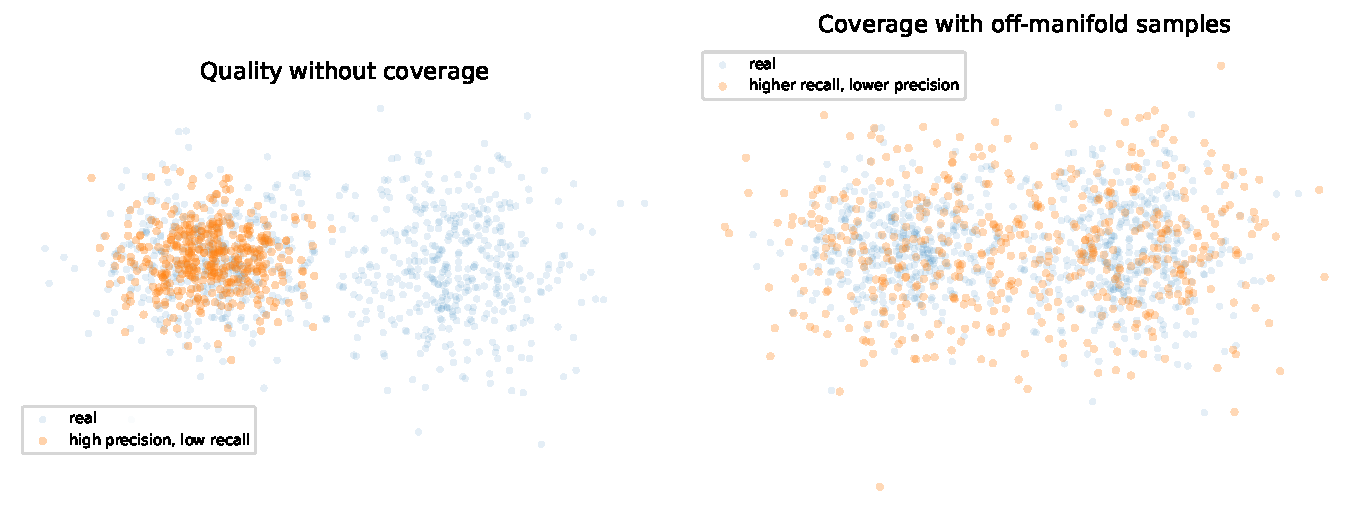
\includegraphics[width=0.96\textwidth]{fig12_22_precision_recall.pdf}
\caption{کیفیت و پوشش دو محور متفاوت‌اند. FID می‌تواند این دو را در یک عدد مخلوط کند.}
\end{figure}

\subsection{حفظ‌کردن داده و nearest-neighbor audit}
برای هر نمونه مصنوعی نزدیک‌ترین نمونه آموزش در چند فضای pixel، perceptual و foundation feature را بیابید. شباهت زیاد به‌تنهایی اثبات کپی نیست، اما باید با عضویت، duplicate detection و تغییرات augmentation بررسی شود. در داده پزشکی یا خصوصی، ارزیابی privacy و memorization ضروری است.

\subsection{ارزیابی شرطی}
برای text-to-image یا label-to-image باید هم fidelity شرط و هم realism/coverage سنجیده شود. CLIPScore می‌تواند alignment را بسنجد ولی نسبت به bias encoder و shortcut حساس است. برای داده علمی، metric دامنه‌ای و downstream task غالباً معتبرتر از Inception عمومی است.

\begin{workshopbox}[FID و KID روی ویژگی مصنوعی]
\begin{latin}
\lstinputlisting[firstline=1,lastline=60]{code/fid_kid_toy.py}
\end{latin}
آزمایش کنید با $N=100,500,5000$ رتبه دو مدل چقدر پایدار است. سپس embedding را با تبدیل خطی و غیرخطی تغییر دهید و نشان دهید metric به فضای ویژگی وابسته است.
\end{workshopbox}

\begin{figure}[H]
\centering
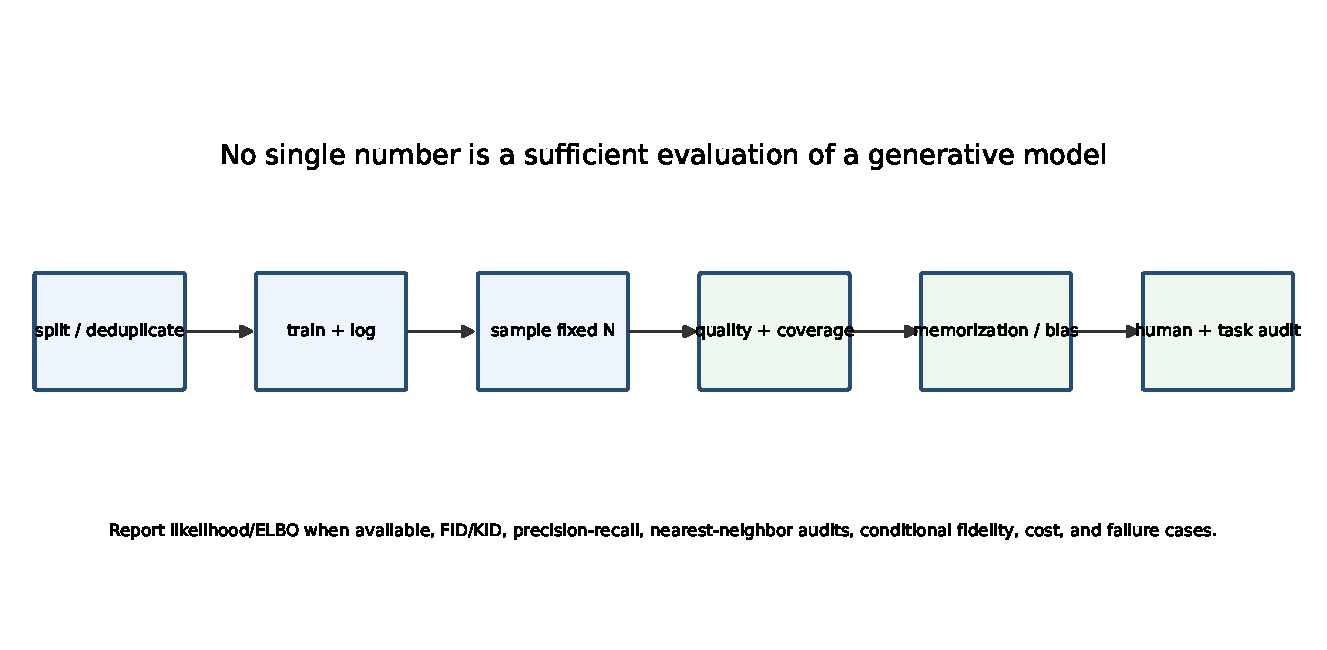
\includegraphics[width=0.98\textwidth]{fig12_24_evaluation.pdf}
\caption{پروتکل ارزیابی چندمحوری. جداسازی داده، تعداد نمونه ثابت و ممیزی شکست قبل از انتخاب بهترین checkpoint ضروری است.}
\end{figure}

\section{پروتکل آزمایش بازتولیدپذیر}
\begin{enumerate}
\item \textbf{داده:} منبع، مجوز، deduplication، رزولوشن، crop و گروه‌های جمعیتی ثبت شود؛
\item \textbf{split:} train/validation/test و هرگونه overlap با pretraining مشخص شود؛
\item \textbf{compute:} GPU/CPU، precision، batch، accumulation، زمان و انرژی تقریبی گزارش شود؛
\item \textbf{آموزش:} seed، optimizer، نرخ‌های دو بازیکن، EMA، augmentation و checkpoint rule ثبت شود؛
\item \textbf{sampling:} تعداد، seed، truncation، temperature، top-k/p و guidance ثابت باشد؛
\item \textbf{metric:} نسخه، feature extractor، preprocessing و reference statistics ذخیره شود؛
\item \textbf{عدم‌قطعیت:} چند run یا bootstrap confidence interval؛
\item \textbf{تصویرها:} نمونه تصادفی و failure gallery، نه فقط cherry-picked؛
\item \textbf{ممیزی:} nearest neighbor، memorization، bias، artifact و conditional failure؛
\item \textbf{کد:} commit، محیط، checksum و log خام نگهداری شود.
\end{enumerate}

\section{کتابخانه‌ها و ابزارهای حرفه‌ای}
\begin{figure}[H]
\centering
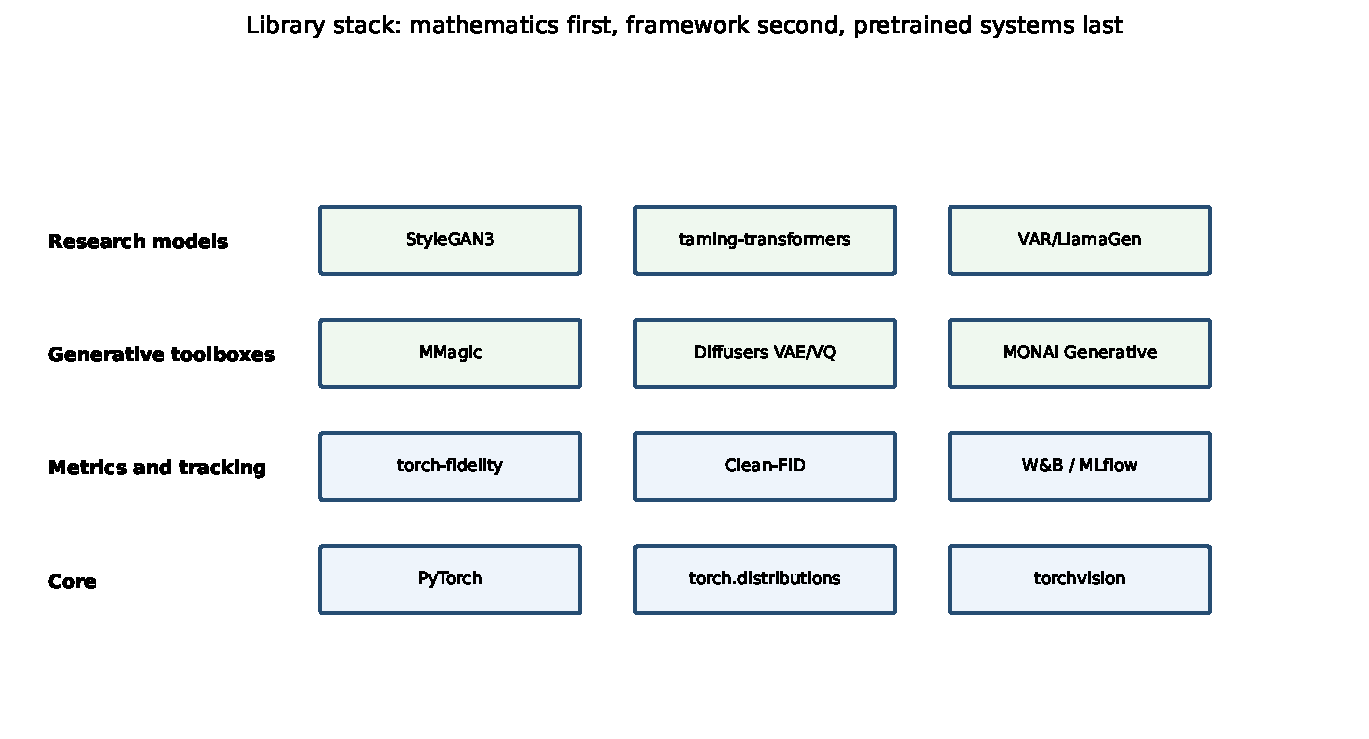
\includegraphics[width=0.96\textwidth]{fig12_23_libraries.pdf}
\caption{پشته کتابخانه‌ای. استفاده از toolbox نباید قراردادهای likelihood، normalization، sampling و metric را پنهان کند.}
\end{figure}

\subsection{PyTorch و torch.distributions}
برای distribution، reparameterized sampling، transformed distribution و constraintها مناسب است. تفاوت \lr{sample()} و \lr{rsample()} باید فهمیده شود؛ دومی pathwise gradient دارد اگر توزیع پشتیبانی کند.

\subsection{torchvision DCGAN tutorial}
برای baseline آموزشی خوب است و pipeline داده، initialization و حلقه دو optimizer را شفاف نشان می‌دهد. برای پژوهش، باید metric، چند seed، augmentation و checkpointing اضافه شود.

\subsection{MMagic}
ابزار OpenMMLab برای generation و restoration با registry، config، runner و model zoo است. مزیت آن مقایسه pipelineهاست؛ خطر آن استفاده از config بدون فهم preprocessing و loss است.

\subsection{مخزن رسمی StyleGAN3}
برای آموزش، تولید، projection و checkpointهای رسمی استفاده می‌شود. قرارداد dataset ZIP، رزولوشن، label metadata، augmentation و گزینه‌های alias-free باید دقیق رعایت شود.

\subsection{Diffusers AutoencoderKL و VQModel}
حتی پیش از فصل diffusion، این کلاس‌ها برای encoder/decoder نهفته مدرن مهم‌اند. scaling factor، latent channels، sample posterior در برابر mode و preprocessing تصویر باید ثبت شوند.

\subsection{ابزار معیار}
\lr{torch-fidelity} و \lr{Clean-FID} اجرای معیار را استانداردتر می‌کنند، اما reference، نسخه وزن و resize همچنان باید ذکر شوند. metric را در environment قفل کنید و آمار واقعی را دوباره استفاده کنید.

\section{انتخاب خانواده مناسب}
{\small
\begin{longtable}{p{25mm}p{25mm}p{25mm}p{25mm}p{25mm}}
\toprule
خانواده & چگالی & نمونه‌گیری & استنباط $z\mid x$ & شکست شاخص \\
\midrule
\lr{VAE} & کران واریاسیونی & موازی و سریع & استنباط تعمیم‌یافته & تاری / فروپاشی پسین \\
\lr{VQ-VAE} با پیشین & وابسته به پیشین & ترتیبی یا چندمرحله‌ای & رمزگذار کوانتیزه & گلوگاه توکن‌ساز و کدبوک \\
\lr{GAN} & ضمنی & یک گذر رو‌به‌جلو & نیازمند وارون‌سازی & ناپایداری و فروپاشی مد \\
خودرگرسیو & دقیق & ترتیبی & معمولاً مستقیم ندارد & کندی نمونه‌گیری / ترتیب مصنوعی \\
جریان نرمال‌ساز & دقیق & دقیق و وارون & دقیق & قید وارون‌پذیری و حافظه \\
انرژی‌محور & تا ثابت $Z$ & \lr{MCMC} & بهینه‌سازی یا نمونه‌گیری & اختلاط ضعیف و ثابت نرمال‌سازی \\
تطبیق جریان & مسیر پیوسته & حل \lr{ODE} & وارون‌سازی با \lr{ODE} & خطای حل‌گر و انتخاب مسیر \\
\bottomrule
\end{longtable}
}

\begin{principlebox}
خانواده را بر اساس نیاز انتخاب کنید، نه شهرت: اگر anomaly likelihood مهم است، density و calibration را بسنجید؛ اگر latency generation مهم است، GAN یا decoder موازی؛ اگر reconstruction و representation مهم است، VAE/VQ؛ اگر sequence infrastructure و scaling مهم است، token AR؛ و اگر transport پیوسته و guidance مهم است، flow/diffusion.
\end{principlebox}

\section{افق ۲۰۲۴ تا ۲۰۲۶}
پژوهش مولد تصویر از دوگانه قدیمی GAN در برابر VAE عبور کرده است. چند روند اصلی:
\begin{itemize}
\item tokenizerهای بسیار فشرده یک‌بعدی مانند TiTok و نسخه‌های adaptive/semantic؛
\item بازگشت مدل‌های خودرگرسیو با LlamaGen، VAR، set/scale autoregression و زیرساخت LLM؛
\item جریان‌های نهفته مقیاس‌پذیر و flow matching؛
\item مدل‌های هیبرید AR--diffusion و tokenizer--foundation feature؛
\item توجه بیشتر به کیفیت dense latent، codebook dimension و rate--distortion؛
\item ارزیابی با feature extractorهای دامنه‌ای و ممیزی حفظ‌کردن داده؛
\item provenance، watermark و تشخیص رسانه مصنوعی به‌عنوان جزء سامانه، نه افزونه بعدی.
\end{itemize}

\begin{figure}[H]
\centering
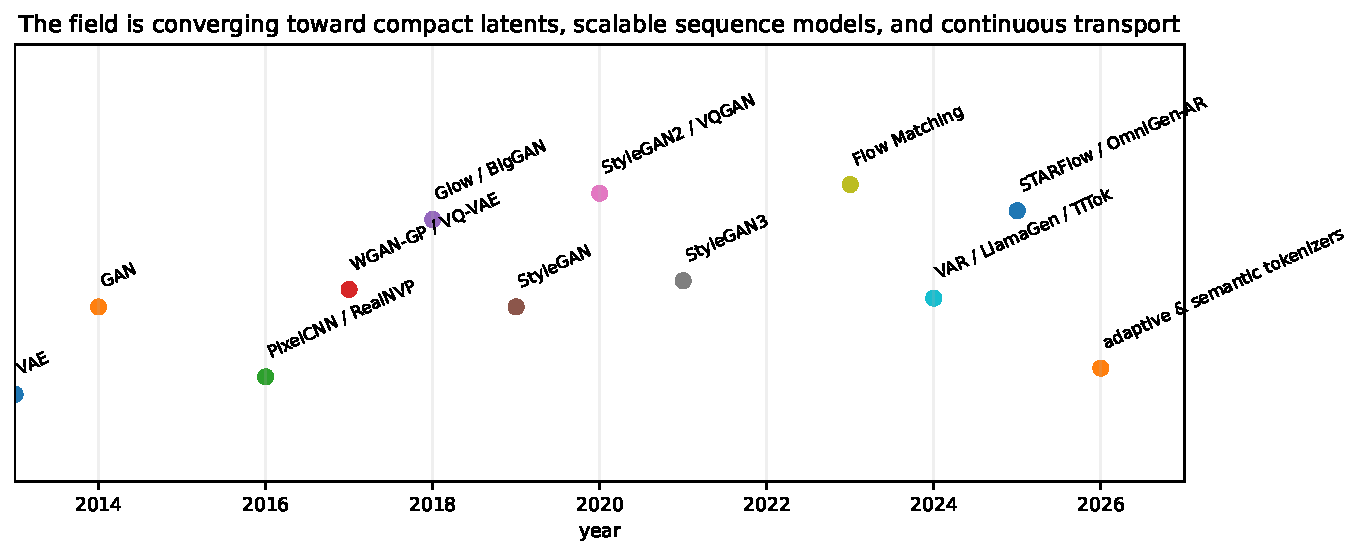
\includegraphics[width=0.98\textwidth]{fig12_25_frontier.pdf}
\caption{خط زمانی مفهومی. مرزهای خانواده‌ها با tokenizerهای فشرده، priorهای ترتیبی و انتقال پیوسته در حال همگرایی‌اند.}
\end{figure}

\begin{futurebox}
فصل سیزدهم مدل‌های انتشار، score، SDE/ODE، denoising، latent diffusion، flow matching و sampling سریع را از ابتدا و با ریاضیات کامل توسعه می‌دهد. در فصل حاضر فقط مفاهیمی آمده‌اند که برای فهم جایگاه آن خانواده در نقشه مولدها لازم است.
\end{futurebox}

\section{الگوریتم‌های مرجع فصل}
\begin{algorithmbox}{الگوریتم ۱۲.۳ ـ VQ-VAE با codebook EMA}
\begin{enumerate}
\item $z_e=E(x)$؛ assignment نزدیک‌ترین code؛
\item decoder روی straight-through quantized latent؛
\item reconstruction و commitment loss؛
\item برای هر code، شمارش و مجموع encoder vectorها؛
\item EMA شمارش و مجموع؛ $e_k\leftarrow m_k/N_k$؛
\item reset کدهای مرده با نمونه encoder؛
\item ثبت perplexity، درصد کد فعال، effective rank و rFID.
\end{enumerate}
\end{algorithmbox}

\begin{algorithmbox}{الگوریتم ۱۲.۴ ـ GAN پایدار با R1 و EMA}
\begin{enumerate}
\item update تمایزگر با logistic/hinge loss؛
\item هر $r$ گام، R1 روی داده واقعی با ضریب تصحیح‌شده؛
\item update مولد با non-saturating یا hinge؛
\item EMA وزن مولد؛
\item augmentation تطبیقی در داده محدود؛
\item هر بازه ثابت، نمونه با seed ثابت و metric با $N$ ثابت؛
\item توقف بر اساس validation metric و coverage، نه training loss تنها.
\end{enumerate}
\end{algorithmbox}

\begin{algorithmbox}{الگوریتم ۱۲.۵ ـ نمونه‌گیری autoregressive با temperature و top-k}
برای $i=1$ تا $N$:
\begin{enumerate}
\item logits $\ell_i=f(c_{<i},condition)$؛
\item $\ell_i\leftarrow\ell_i/T$؛
\item همه logits خارج top-k را $-\infty$ کنید؛
\item $c_i\sim\operatorname{Categorical}(\softmax(\ell_i))$؛
\item token را به cache اضافه کنید؛
\item در پایان، decoder tokenها را به تصویر تبدیل کند.
\end{enumerate}
temperature کم precision را بالا و diversity را کم می‌کند؛ اثر باید گزارش شود.
\end{algorithmbox}

\begin{algorithmbox}{الگوریتم ۱۲.۶ ـ آموزش RealNVP با maximum likelihood}
\begin{enumerate}
\item dequantize و logit transform با correction Jacobian؛
\item $z=f_\theta(x)$ و logdet همه couplingها؛
\item $\log p(x)=\log p_Z(z)+\sum logdet$؛
\item منفی میانگین log-likelihood را کمینه کنید؛
\item آزمون وارون و logdet عددی در هر تغییر معماری؛
\item bits/dim و نمونه prior را هر دو گزارش کنید.
\end{enumerate}
\end{algorithmbox}

\section{آزمایش‌های پیشنهادی فصل}
\begin{enumerate}
\item \textbf{VAE rate--distortion:} $\beta\in\{0.1,0.5,1,2,4\}$؛ recon، KL، active units و FID نمونه prior.
\item \textbf{Posterior collapse:} decoder ضعیف/قوی، KL warm-up و free bits.
\item \textbf{VQ codebook:} اندازه codebook، بعد code، EMA و reset؛ rFID در برابر perplexity.
\item \textbf{GAN objective:} minimax، non-saturating، hinge و WGAN-GP روی مخلوط مدها.
\item \textbf{Lipschitz:} clipping، GP و spectral norm؛ norm gradient در فضای ورودی.
\item \textbf{Data-limited GAN:} بدون augmentation، DiffAugment و ADA.
\item \textbf{Truncation:} منحنی precision--recall و FID در چند $\psi$.
\item \textbf{Autoregressive order:} raster، serpentine و coarse-to-fine.
\item \textbf{Tokenizer frontier:} token count در برابر reconstruction و زمان generation.
\item \textbf{Flow:} تعداد coupling و نوع permutation؛ likelihood در برابر sample quality.
\item \textbf{Metric stability:} FID/KID با تعداد نمونه و extractor مختلف.
\item \textbf{Memorization audit:} نزدیک‌ترین همسایه train/test برای چند checkpoint.
\end{enumerate}

\section{پروژه‌های پایان فصل}
\begin{enumerate}
\item \textbf{آزمایشگاه VAE تشخیصی:} dashboard نرخ، اعوجاج، active units و posterior collapse.
\item \textbf{VQ tokenizer برای تصاویر صنعتی:} مقایسه codebook، residual VQ و tokenizer پیوسته.
\item \textbf{GAN داده کم:} StyleGAN2-ADA یا baseline کوچک با ممیزی overfit.
\item \textbf{ترجمه تصویر علمی:} pix2pix/CycleGAN با قید حفظ ساختار و آزمون hallucination.
\item \textbf{مولد توکنی کوچک:} VQ-VAE + Transformer روی تصاویر $32\times32$.
\item \textbf{RealNVP/Glow آموزشی:} چگالی، sampling، interpolation و OOD paradox.
\item \textbf{سامانه معیار:} FID، KID، precision/recall، nearest neighbor و گزارش HTML.
\item \textbf{مطالعه خانواده‌ها:} compute-matched VAE، GAN و AR با بودجه پارامتر و زمان یکسان.
\end{enumerate}

\section{تمرین‌های نظری}
\begin{enumerate}
\item هویت دقیق log-likelihood، ELBO و variational gap را اثبات کنید.
\item KL دو Gaussian قطری را از تعریف استخراج کنید.
\item نشان دهید MSE معادل منفی log-likelihood Gaussian با واریانس ثابت است.
\item برای Gaussian decoder با واریانس آموختنی، تابع زیان کامل را بنویسید.
\item gradient بازپارامتردهی برای $h(z)=z^2$ را تحلیلی و مونت‌کارلو مقایسه کنید.
\item aggregate posterior را تعریف و تفاوت WAE با VAE را توضیح دهید.
\item تمایزگر بهینه GAN را استخراج و مقدار $V(D^*,G)$ را به JS تبدیل کنید.
\item توضیح دهید چرا non-saturating loss همان divergence ساده را دقیقاً کمینه نمی‌کند.
\item دوگان Wasserstein-1 را بیان و نقش Lipschitz را توضیح دهید.
\item یک مثال بسازید که weight clipping ظرفیت critic را محدود کند.
\item logdet coupling affine را استخراج کنید.
\item رابطه میان MAF و IAF را از وارون‌کردن ترتیب توضیح دهید.
\item نشان دهید masked convolution نوع A leakage ندارد.
\item برای تصویر RGB یک فاکتورگیری علّی میان پیکسل و کانال طراحی کنید.
\item bias برآوردگر FID را با شبیه‌سازی بررسی کنید.
\item نشان دهید truncation می‌تواند recall را کاهش دهد.
\item یک counterexample برای تفسیر likelihood به‌عنوان OOD score بسازید.
\item تفاوت codebook perplexity و effective rank را توضیح دهید.
\item چرا cycle consistency شناساپذیری معنایی را تضمین نمی‌کند؟
\item flow matching و maximum likelihood CNF را از نظر نیاز به حل ODE مقایسه کنید.
\end{enumerate}

\section{تمرین‌های کدنویسی}
\begin{enumerate}
\item به VAE، convolutional encoder/decoder اضافه کنید.
\item KL per-dimension و active units را log کنید.
\item free bits و cyclical annealing را پیاده کنید.
\item VQ با EMA و reset کد مرده بسازید.
\item gradient penalty را با finite difference کنترل کنید.
\item spectral normalization را با power iteration از صفر پیاده کنید.
\item روی GAN، occupancy هشت مد و entropy آن را رسم کنید.
\item R1 را lazy اجرا و ضریب درست را آزمون کنید.
\item masked convolution را برای RGB channel ordering توسعه دهید.
\item KV-cache ساده برای Transformer token prior بسازید.
\item RealNVP را روی two-moons آموزش دهید.
\item logdet analytic و autograd Jacobian را مقایسه کنید.
\item FID را با bootstrap interval گزارش کنید.
\item precision/recall توزیعی را روی feature مصنوعی پیاده کنید.
\item nearest-neighbor montage train/test تولید کنید.
\end{enumerate}

\begin{videobox}
پیشنهاد فصل برای \textbf{۱۰۴ ویدئوی ۱۵ دقیقه‌ای}:
\begin{enumerate}
\item ویدئوهای ۱--۸: تعریف مدل مولد، pushforward، likelihood و واگرایی‌ها؛
\item ۹--۲۴: خودرمزگذار، ELBO، بازپارامتردهی، likelihood مشاهده و کد VAE؛
\item ۲۵--۳۴: posterior collapse، $\beta$-VAE، IWAE، WAE و VAE سلسله‌مراتبی؛
\item ۳۵--۴۴: VQ-VAE، codebook، VQGAN و آزمایش tokenizer؛
\item ۴۵--۶۲: GAN، تمایزگر بهینه، زیان‌ها، دینامیک، collapse، WGAN و regularization؛
\item ۶۳--۷۴: DCGAN، conditional، pix2pix، CycleGAN، BigGAN و StyleGAN؛
\item ۷۵--۸۴: PixelCNN، likelihood پیکسل، token prior، MaskGIT، LlamaGen و VAR؛
\item ۸۵--۹۳: RealNVP، Glow، MAF/IAF، dequantization، CNF و flow matching؛
\item ۹۴--۹۸: EBM، Langevin و score؛
\item ۹۹--۱۰۲: معیارها، ممیزی، کتابخانه‌ها و بازتولید؛
\item ۱۰۳--۱۰۴: ارائه پروژه و پل به diffusion.
\end{enumerate}
\end{videobox}

\section{پرامپت جامع برای Codex}
\begin{codecontract}
کد باید از متن علمی تبعیت کند: هر loss با رابطه فصل، هر metric با نسخه و preprocessing، هر نمودار با CSV خام و هر checkpoint با config و seed همراه باشد. خروجی تصویری بدون log عددی نتیجه علمی محسوب نمی‌شود.
\end{codecontract}

\begin{latin}
\begin{lstlisting}
Act as a senior research engineer in deep generative image modeling.
Build a reproducible PyTorch laboratory comparing six families under a
matched compute budget: VAE, VQ-VAE, non-saturating GAN, WGAN-GP,
PixelCNN/token autoregressive model, and RealNVP.

Requirements:
1. Use a single configuration system and deterministic seeds.
2. Provide synthetic 2-D sanity tests before image experiments.
3. Separate tokenizer reconstruction quality from token-prior quality.
4. Log reconstruction, KL/rate, active units, code usage/perplexity,
   critic gradients, mode occupancy, likelihood/bits-dim, FID, KID,
   precision-recall, latency, memory, and nearest-neighbor audits.
5. Implement unit tests for VAE reparameterization shapes, masked-conv
   causality, flow invertibility/log-det, gradient penalty, and metric
   invariance to batch partitioning.
6. Never invent results. Every table must be generated from CSV/JSON logs.
7. Save random and failure samples, not only curated samples.
8. Export an experiment card with dataset license, preprocessing,
   model commit, hardware, runtime, seeds, sampling parameters, and caveats.
9. Include README commands for CPU smoke tests and GPU full runs.
10. Produce a LaTeX-ready table and figure manifest.
\end{lstlisting}
\end{latin}

\begin{summarybox}
\begin{itemize}
\item VAE یک مدل متغیر نهفته با استنباط amortized و کران واریاسیونی است؛ reconstruction و KL معنای احتمالاتی دارند.
\item VQ-VAE تصویر را به الفبای گسسته تبدیل می‌کند؛ کیفیت و استفاده codebook باید مستقل از prior سنجیده شود.
\item GAN یک بازی توزیعی با چگالی ضمنی است؛ کیفیت نمونه بالا می‌تواند با پوشش ناقص همراه باشد.
\item WGAN و regularizationهای Lipschitz هندسه gradient را بهبود می‌دهند ولی جای عیب‌یابی را نمی‌گیرند.
\item مدل خودرگرسیو likelihood دقیق دارد، اما ترتیب و sampling متوالی هزینه‌زاست؛ tokenization و next-scale این هزینه را تغییر می‌دهند.
\item جریان نرمال‌ساز likelihood و inversion دقیق را با قید وارون‌پذیری و determinant قابل محاسبه مبادله می‌کند.
\item مدل انرژی‌محور انعطاف‌پذیر است، ولی sampling و ثابت نرمال‌سازی دشوارند.
\item هیچ معیار واحدی کافی نیست؛ likelihood، quality، coverage، memorization، fidelity شرطی و compute باید با هم گزارش شوند.
\end{itemize}
\end{summarybox}

\section*{منابع منتخب و مسیر مطالعه}
\addcontentsline{toc}{section}{منابع منتخب و مسیر مطالعه}
\begin{latin}
\begin{thebibliography}{99}
\bibitem{aevb} D. P. Kingma and M. Welling, ``Auto-Encoding Variational Bayes,'' ICLR, 2014.
\bibitem{vaeintro} D. P. Kingma and M. Welling, ``An Introduction to Variational Autoencoders,'' Foundations and Trends in Machine Learning, 2019.
\bibitem{iwae} Y. Burda, R. Grosse, and R. Salakhutdinov, ``Importance Weighted Autoencoders,'' ICLR, 2016.
\bibitem{betavae} I. Higgins et al., ``beta-VAE: Learning Basic Visual Concepts with a Constrained Variational Framework,'' ICLR, 2017.
\bibitem{factorvae} H. Kim and A. Mnih, ``Disentangling by Factorising,'' ICML, 2018.
\bibitem{infovae} S. Zhao, J. Song, and S. Ermon, ``InfoVAE: Information Maximizing Variational Autoencoders,'' AAAI, 2019.
\bibitem{wae} I. Tolstikhin et al., ``Wasserstein Auto-Encoders,'' ICLR, 2018.
\bibitem{nvae} A. Vahdat and J. Kautz, ``NVAE: A Deep Hierarchical Variational Autoencoder,'' NeurIPS, 2020.
\bibitem{vdvae} R. Child, ``Very Deep VAEs Generalize Autoregressive Models and Can Outperform Them on Images,'' ICLR, 2021.
\bibitem{vqvae} A. van den Oord, O. Vinyals, and K. Kavukcuoglu, ``Neural Discrete Representation Learning,'' NeurIPS, 2017.
\bibitem{vqgan} P. Esser, R. Rombach, and B. Ommer, ``Taming Transformers for High-Resolution Image Synthesis,'' CVPR, 2021.
\bibitem{gan} I. Goodfellow et al., ``Generative Adversarial Nets,'' NeurIPS, 2014.
\bibitem{dcgan} A. Radford, L. Metz, and S. Chintala, ``Unsupervised Representation Learning with Deep Convolutional GANs,'' ICLR, 2016.
\bibitem{fgan} S. Nowozin, B. Cseke, and R. Tomioka, ``f-GAN: Training Generative Neural Samplers using Variational Divergence Minimization,'' NeurIPS, 2016.
\bibitem{wgan} M. Arjovsky, S. Chintala, and L. Bottou, ``Wasserstein GAN,'' ICML, 2017.
\bibitem{wgangp} I. Gulrajani et al., ``Improved Training of Wasserstein GANs,'' NeurIPS, 2017.
\bibitem{spectral} T. Miyato et al., ``Spectral Normalization for Generative Adversarial Networks,'' ICLR, 2018.
\bibitem{ttur} M. Heusel et al., ``GANs Trained by a Two Time-Scale Update Rule Converge to a Local Nash Equilibrium,'' NeurIPS, 2017.
\bibitem{biggan} A. Brock, J. Donahue, and K. Simonyan, ``Large Scale GAN Training for High Fidelity Natural Image Synthesis,'' ICLR, 2019.
\bibitem{stylegan} T. Karras, S. Laine, and T. Aila, ``A Style-Based Generator Architecture for Generative Adversarial Networks,'' CVPR, 2019.
\bibitem{stylegan2} T. Karras et al., ``Analyzing and Improving the Image Quality of StyleGAN,'' CVPR, 2020.
\bibitem{ada} T. Karras et al., ``Training Generative Adversarial Networks with Limited Data,'' NeurIPS, 2020.
\bibitem{stylegan3} T. Karras et al., ``Alias-Free Generative Adversarial Networks,'' NeurIPS, 2021.
\bibitem{pix2pix} P. Isola et al., ``Image-to-Image Translation with Conditional Adversarial Networks,'' CVPR, 2017.
\bibitem{cyclegan} J.-Y. Zhu et al., ``Unpaired Image-to-Image Translation using Cycle-Consistent Adversarial Networks,'' ICCV, 2017.
\bibitem{pixelcnn} A. van den Oord et al., ``Conditional Image Generation with PixelCNN Decoders,'' NeurIPS, 2016.
\bibitem{pixelcnnpp} T. Salimans et al., ``PixelCNN++: Improving the PixelCNN with Discretized Logistic Mixture Likelihood and Other Modifications,'' ICLR, 2017.
\bibitem{realnvp} L. Dinh, J. Sohl-Dickstein, and S. Bengio, ``Density Estimation using Real NVP,'' ICLR, 2017.
\bibitem{maf} G. Papamakarios, T. Pavlakou, and I. Murray, ``Masked Autoregressive Flow for Density Estimation,'' NeurIPS, 2017.
\bibitem{iaf} D. P. Kingma et al., ``Improved Variational Inference with Inverse Autoregressive Flow,'' NeurIPS, 2016.
\bibitem{glow} D. P. Kingma and P. Dhariwal, ``Glow: Generative Flow with Invertible 1x1 Convolutions,'' NeurIPS, 2018.
\bibitem{ffjord} W. Grathwohl et al., ``FFJORD: Free-form Continuous Dynamics for Scalable Reversible Generative Models,'' ICLR, 2019.
\bibitem{flowmatching} Y. Lipman et al., ``Flow Matching for Generative Modeling,'' ICLR, 2023.
\bibitem{fid} M. Heusel et al., ``GANs Trained by a Two Time-Scale Update Rule...,'' NeurIPS, 2017.
\bibitem{kid} M. Binkowski et al., ``Demystifying MMD GANs,'' ICLR, 2018.
\bibitem{pr} M. Sajjadi et al., ``Assessing Generative Models via Precision and Recall,'' NeurIPS, 2018.
\bibitem{ipr} T. Kynkaanniemi et al., ``Improved Precision and Recall Metric for Assessing Generative Models,'' NeurIPS, 2019.
\bibitem{var} K. Tian et al., ``Visual Autoregressive Modeling: Scalable Image Generation via Next-Scale Prediction,'' NeurIPS, 2024.
\bibitem{llamagen} P. Sun et al., ``Autoregressive Model Beats Diffusion: Llama for Scalable Image Generation,'' 2024.
\bibitem{titok} Q. Yu et al., ``An Image is Worth 32 Tokens for Reconstruction and Generation,'' NeurIPS, 2024.
\bibitem{omnigenar} ``OmniGen-AR: AutoRegressive Any-to-Image Generation,'' NeurIPS, 2025.
\bibitem{starflow} ``Scaling Latent Normalizing Flows for High-Resolution Image Synthesis,'' NeurIPS, 2025.
\bibitem{vqwarmup} X. Zhao et al., ``Continuous First, Discrete Later: VQ-VAEs Without Dimensional Collapse,'' 2026.
\bibitem{pytorchtutorial} PyTorch Contributors, ``DCGAN Tutorial,'' official documentation, accessed July 2026.
\bibitem{diffusersvae} Hugging Face Contributors, ``AutoencoderKL and VQModel Documentation,'' official Diffusers documentation, accessed July 2026.
\bibitem{mmagic} OpenMMLab Contributors, ``MMagic Documentation and Model Zoo,'' accessed July 2026.
\bibitem{styleganrepo} NVIDIA Research, ``StyleGAN3 Official PyTorch Implementation,'' accessed July 2026.
\end{thebibliography}
\end{latin}

\appendix
\chapter{راهنمای ساخت، اجرا و بازتولید}
\section{ساخت PDF}
\begin{latin}
\begin{lstlisting}
xelatex image_processing_next_decade_ch12_fa.tex
xelatex image_processing_next_decade_ch12_fa.tex
\end{lstlisting}
\end{latin}

\section{محیط پایتون}
\begin{latin}
\begin{lstlisting}
python -m venv .venv
source .venv/bin/activate       # Windows: .venv\Scripts\activate
python -m pip install --upgrade pip
python -m pip install -r requirements.txt
\end{lstlisting}
\end{latin}

\section{تولید شکل‌ها}
\begin{latin}
\begin{lstlisting}
python generate_figures.py
\end{lstlisting}
\end{latin}
تمام نمودارهای عددی فصل آموزشی و بازتولیدپذیرند و به‌عنوان نتیجه تجربی مقاله معرفی نشده‌اند.

\section{Smoke test کدها}
\begin{latin}
\begin{lstlisting}
python code/vae_minimal.py
python code/vq_vae_minimal.py
python code/gan_minimal.py
python code/wgan_gp_minimal.py
python code/realnvp_2d.py
python code/pixelcnn_mask.py
python code/fid_kid_toy.py
python code/latent_interpolation.py
python code/flow_matching_2d.py
\end{lstlisting}
\end{latin}
خروجی اجرای کنترل‌شده در \lr{outputs/smoke\_test.txt} ذخیره شده است.

\section{پیش‌پرواز علمی}
\begin{enumerate}
\item خروجی‌های نمونه با seed و checkpoint مشخص باشند؛
\item بهترین نمونه‌ها جدا از نمونه تصادفی برچسب بخورند؛
\item metric روی تعداد نمونه و preprocessing ثابت محاسبه شود؛
\item tokenizer و prior جداگانه ارزیابی شوند؛
\item train/test nearest neighbor هر دو بررسی شوند؛
\item چند seed یا bootstrap uncertainty ارائه شود؛
\item failure، collapse و subgroup ضعیف پنهان نشوند؛
\item license داده و وزن‌ها ثبت شود.
\end{enumerate}

\end{document}
